Um die Funktionsweise beider Methoden zu belegen wurden diese sowohl auf ihre Robustheit als auch auf ihre Performance getestet. In diesem Kapitel wird zunächst das zum Testen verwendete Setup erläutert. Weiterhin werden die einzelnen durchgeführten Tests sowie die erlangten Ergebnisse beschrieben. Zuletzt erfolgt eine Diskussion der erlangten Werte sowie eine Gegenüberstellung beider Algorithmen.

%%%%%%%%%%%%%%%%%%%%%%%%%%%%%%%%%%%%%%%%%%%%%%%%%%%%%%%%%
% ---------------------- SECTION ---------------------- %
%%%%%%%%%%%%%%%%%%%%%%%%%%%%%%%%%%%%%%%%%%%%%%%%%%%%%%%%%
\section{Testsetup}
\label{sec:test_setup}

Bei der Durchführung der Tests befinden sich die Kameras statisch im Raum. Um sicher zu stellen, dass sich die Position der Kameras während der einzelnen Versuche nicht verändert wurden diese auf einer Eisenplatte mittels eines Laborstativs magnetisch befestigt (siehe Abbildung \ref{fig:setup}) Die potentiellen Testhindernisse werden innerhalb der zu erkennenden Reichweite platziert, wobei die Ausrichtung der Hindernisse teils zufällig, teils bewusst in kritischen Positionen erfolgt um ein reales Anwendungsszenario zu simulieren. Ein aufgenommenes Testset besteht dabei aus einem Stereobildpaar, der Disparitätenkarte, einer kompletten Punktwolke dieser um etwaige Fehler der Algorithmen leichter erkennen zu können, sowie den einzelnen erkannten Hindernispunktwolken. Weiterhin werden diverse Parameter gespeichert, wie die Anzahl der erkannten Hinderniselemente sowie deren Disparitäten.\\

\begin{figure}[h]
	\centering
	\begin{tabular}{ccc}
		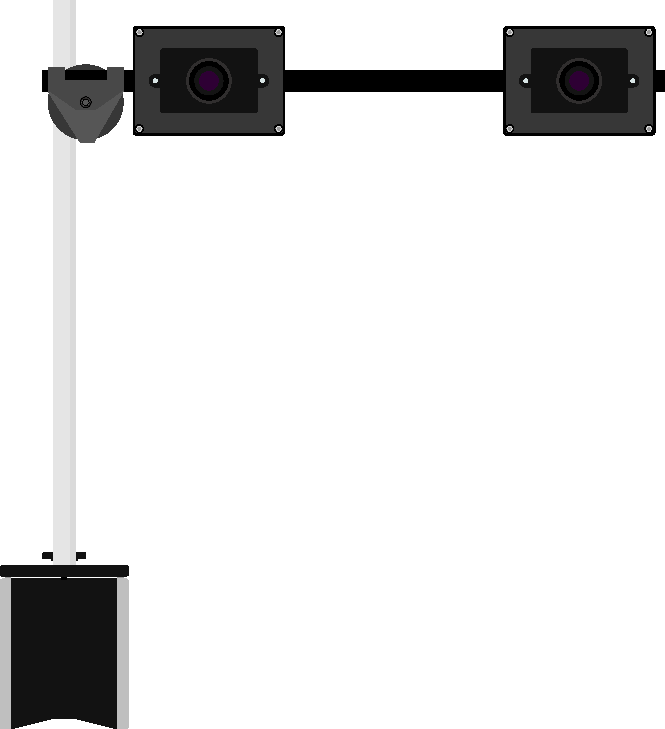
\includegraphics[height=5cm]{img/camera_setup_front} & 
		\quad \quad \quad \quad \quad \quad \quad & 
		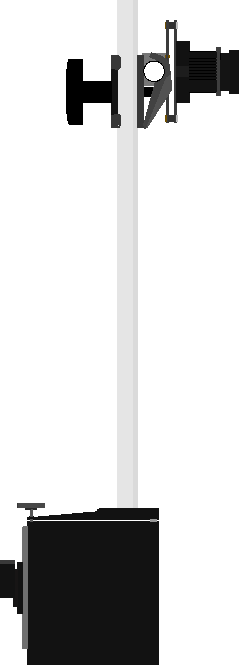
\includegraphics[height=5cm]{img/camera_setup_side} \\
		(a) & & (b)
	\end{tabular}
	\caption{Ansicht des Kamera frontal (a) und von der Seite (b).}
	\label{fig:setup}
\end{figure}

\noindent
Der zu erkennende Bereich wurde auf $0,2$ bis $1,5$ Meter definiert. Dies entspricht einem Szenario in dem das System auch aufgrund der hohen Framerate der Erkennung angewendet werden kann. Die maximale Geschwindigkeit des Pelican beträgt $16 m/s$. Bei einer Framerate von 40 Bildern pro Sekunde ergibt sich eine zurückgelegte Distanz von $16/40=0.4 m$ je Einzelbild. Da das System für die Verwendung in Innenräumen konzipiert ist, ist auch die maximale Geschwindigkeit deutlich geringer. Bei einer angenommenen Geschwindigkeit von $4 m/s$ ergibt sich ein Einzelbild alle 10 cm. Dies reicht für etwaige Manöver zur Vermeidung eines Hindernis aus. Eine Erweiterung dessen auf beispielsweise $2.0$ Meter wurde im Rahmen der Tests nicht durchgeführt, da in vorhergehenden Experimenten bereits festgestellt wurde, dass mit dem vorliegenden Setup robust Disparitätenkarten und daraus entsprechend gute Distanzwerte berechnet werden können \cite{hilleralhallak}. Das nach der Anwendung der ROI auf die Disparitätenkarte verbleibende Sichtfeld (siehe \ref{sec:preprocessing}) beträgt $50^{\circ}$ auf horizontaler Achse und $38^{\circ}$ vertikal. Dabei ist dieses in Abhängigkeit der verwendeten Parameter breiter oder schmaler. Dies ist in Abbildung \ref{fig:field_of_view} visualisiert.
	
	\begin{figure}[h]
		\centering
		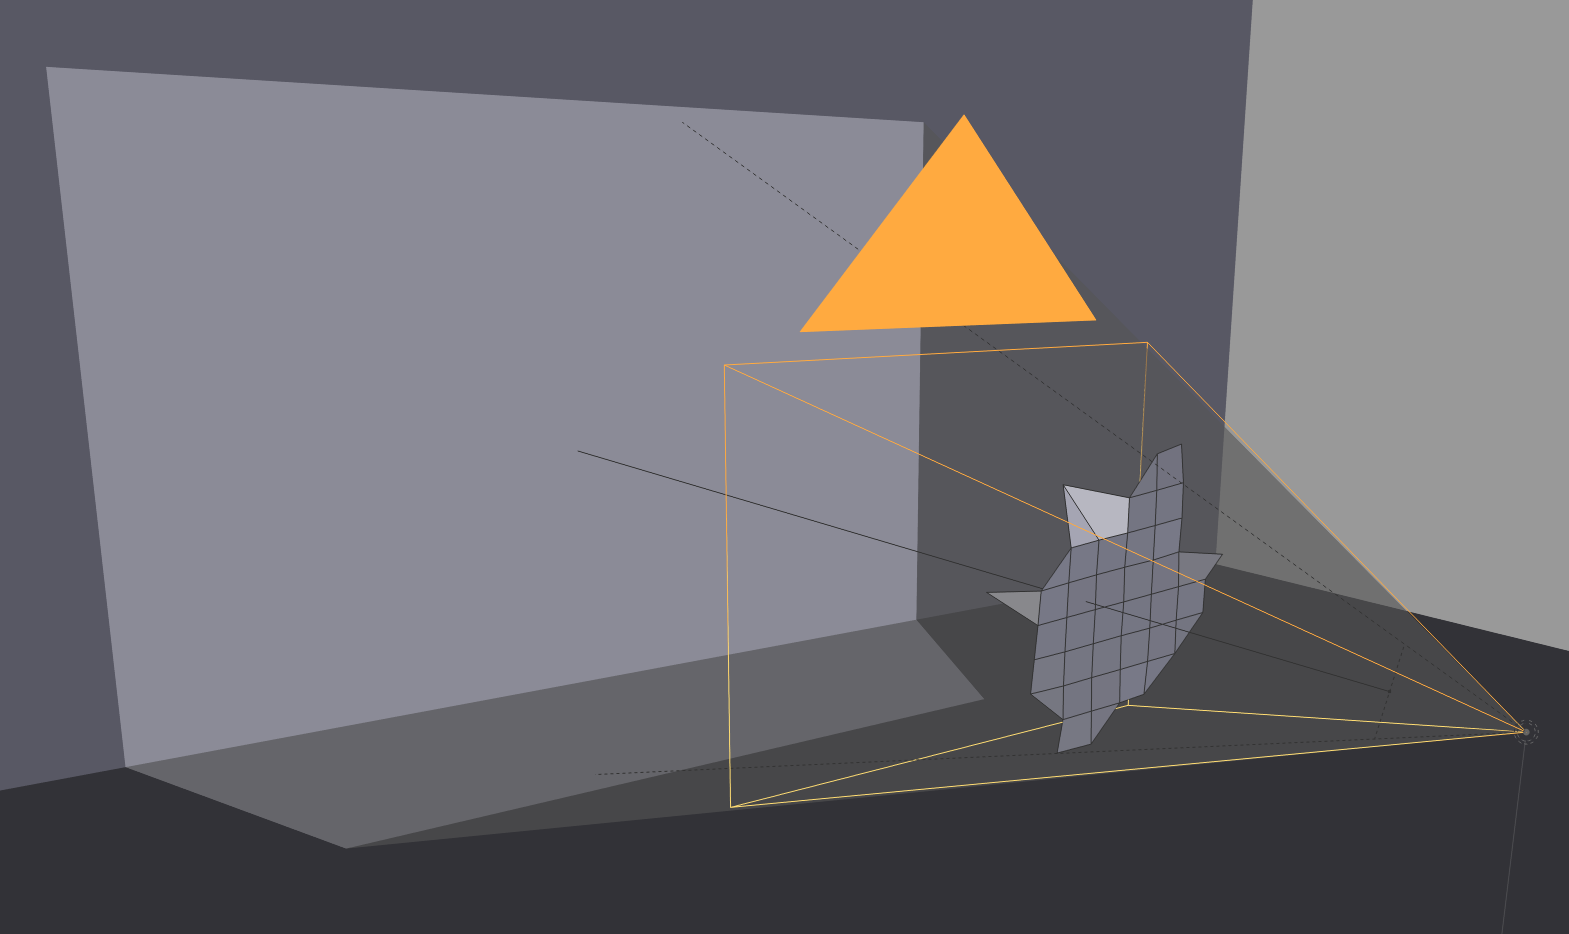
\includegraphics[width=8cm]{img/viewport}
		\caption{Im Bild ist das nach der Rektifizierung sowie Beschneidung der ROI erhaltene Sichtfeld visualisiert. Das Mesh innerhalb des Kamera Frustums repräsentiert die gerenderte Pointcloud eines Hindernisses}
		\label{fig:field_of_view}
	\end{figure}

\noindent
Ein aufgenommenes Testset besteht aus jeweils 12 Testbildern. Für jede Methode wurden drei verschiedene Hindernisgrößen getestet, groß, mittel und kleine Hindernisse (dargestellt in Abbildung \ref{fig:test_obstacles}. Anhand dieser wird ausgewertet welche minimale, maximale sowie mittlere Disparität, und daraus resultierende Distanz erkannt wird. Um eine bessere Vorstellung der Größe der verwendeten Hindernisse zu erhalten werden die Dimensionen dieser in Tabelle \ref{tbl:obstacle_sizes} aufgeführt. Ein großer Abstand zwischen Hindernis 2 und 3 ist dabei gewünscht um die Erkennung sehr kleiner Hindernisse zu untersuchen. \\

\begin{figure}[h]
	\centering
	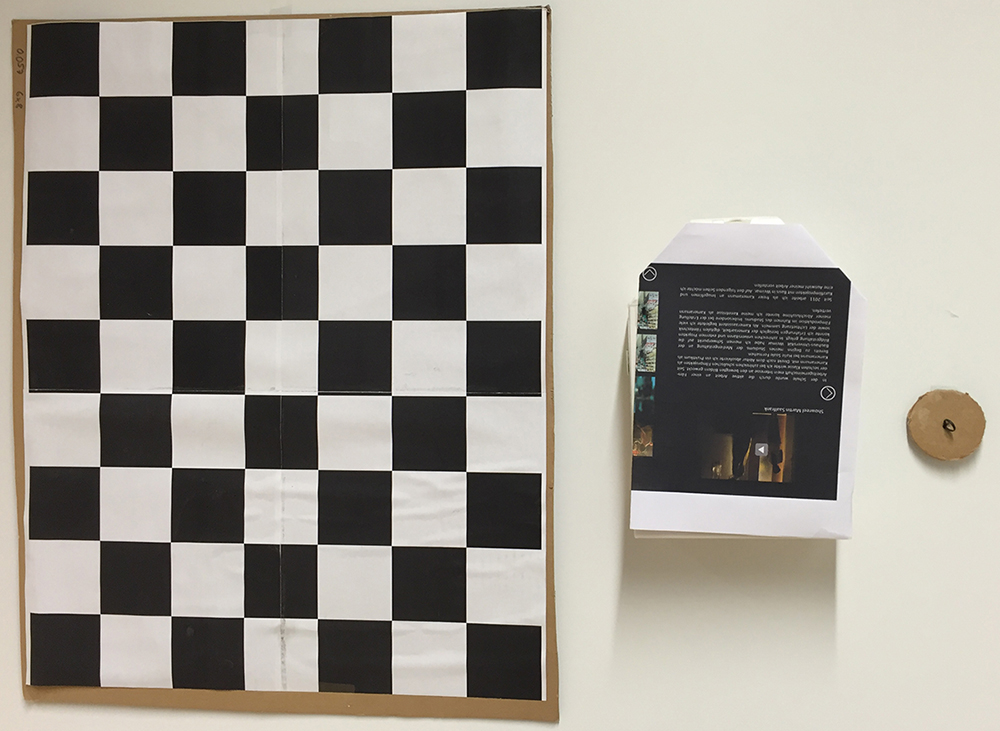
\includegraphics[width=6cm]{img/test_obstacles}
	\caption{Verwendete Testhindernisse, die Kantenlänge eines Quadrates des linken Hindernis beträgt 5.5 cm}
	\label{fig:test_obstacles}
\end{figure}

\begin{table}[h]
\centering
\begin{tabular}{|l|c|c|c|c|}
\hline
Hindernis   & Radius ($cm$) & Länge ($cm$)& Breite ($cm$)& Fläche ($cm^2$)\\
\hline
1 (Groß)   	&   -    & 53.5  & 43.0   & 2300.5 \\
\hline
2 (Mittel) 	& 	-    & 16.0  & 14.5   & 232.0\\
\hline
3 (Klein)	&  2.5	 &   -   &   -    & 19.6 \\
\hline	
\end{tabular}
\caption{Maße der verschiedenen genutzten Hindernisse}
\label{tbl:obstacle_sizes}
\end{table}

\noindent
Weitere Tests beinhalten die Erkennung kleiner Hindernisse unter Veränderung der SGBM Parameter. Dabei wird unter anderem untersucht ob beispielsweise eine verringerte Blockgröße Einfluss auf die Erkennung kleiner Bereiche nimmt. Da die \emph{Samplepoint Detection} den Radius als modifizierbaren Parameter mit sich bringt, wird auch dahingehend untersucht inwiefern die Wahl eines anderen Radius die Ergebnisse der Erkennung beeinflusst. Zudem wird die Funktionsfähigkeit der Methoden bei reflektierenden sowie durchsichtigen Flächen untersucht.\\

\noindent
Die aufgenommenen Disparitätenkarten sind in der Darstellung aufgrund der Normalisierung und teilweise sehr hohen Disparitäten (Ausreißer) oft sehr dunkel. Deshalb wurden für Zwecke der Visualisierung der Kontrast einzelner Disparitätenkarten angepasst/optimiert. Weitere Modifikationen der Bilder wurden nicht vorgenommen.


%%%%%%%%%%%%%%%%%%%%%%%%%%%%%%%%%%%%%%%%%%%%%%%%%%%%%%%%%
% ---------------------- SECTION ---------------------- %
%%%%%%%%%%%%%%%%%%%%%%%%%%%%%%%%%%%%%%%%%%%%%%%%%%%%%%%%%
\section{Durchführung und Ergebnisse}

\subsection{Robustheit}
\label{sec:robustness_evaluation}

Hinsichtlich der Robustheit werden beide Algorithmen nach demselben Schema untersucht. Während der Tests wurde für jedes aufgenommene Einzelbild die reale Distanz gemessen. Der dabei verwendete Referenzpunkt befand sich in der Mitte des zu erkennenden Hindernisses, da diese nicht zwangsläufig orthogonal zur Bildebene platziert wurden. Die berechnete Distanz entspricht der mittleren Distanz welche sich aus allen erkannten Bereichen eines Bildes zusammensetzt.\\

\noindent
Während der Aufnahme sind die jeweiligen Einzelbilder der linken und rechten Kamera sowie die berechnete Disparitätenkarte sichtbar. Zudem ist ein weiterer Anzeigemodus verfügbar welcher die gefundenen Hindernisse innerhalb der Tiefenkarte markiert (siehe Abbildung \ref{fig:test_viewing}). Weiterhin kann jede erstellte Hindernis-Pointcloud im Nachhinein gerendert werden um einen Überblick über die Ergebnisse des Algorithmus zu erhalten.

\begin{figure}[h]
	\centering
	\begin{tabular}{cc}
	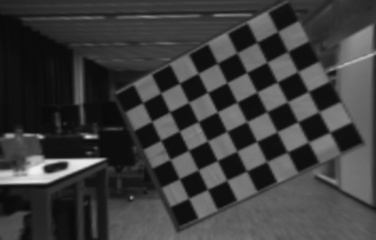
\includegraphics[width=5.5cm]{img/evaluation/test_set/_test_3_left}&
	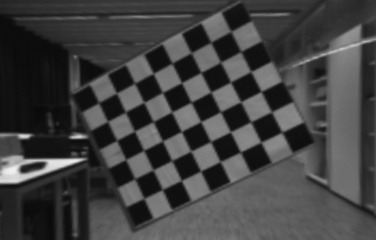
\includegraphics[width=5.5cm]{img/evaluation/test_set/_test_3_right}\\
	(a) linkes Kamerabild & (b) rechtes Kamerabild\\
	
\includegraphics[width=5.5cm]{img/evaluation/test_set/_test_3_disparity}&
    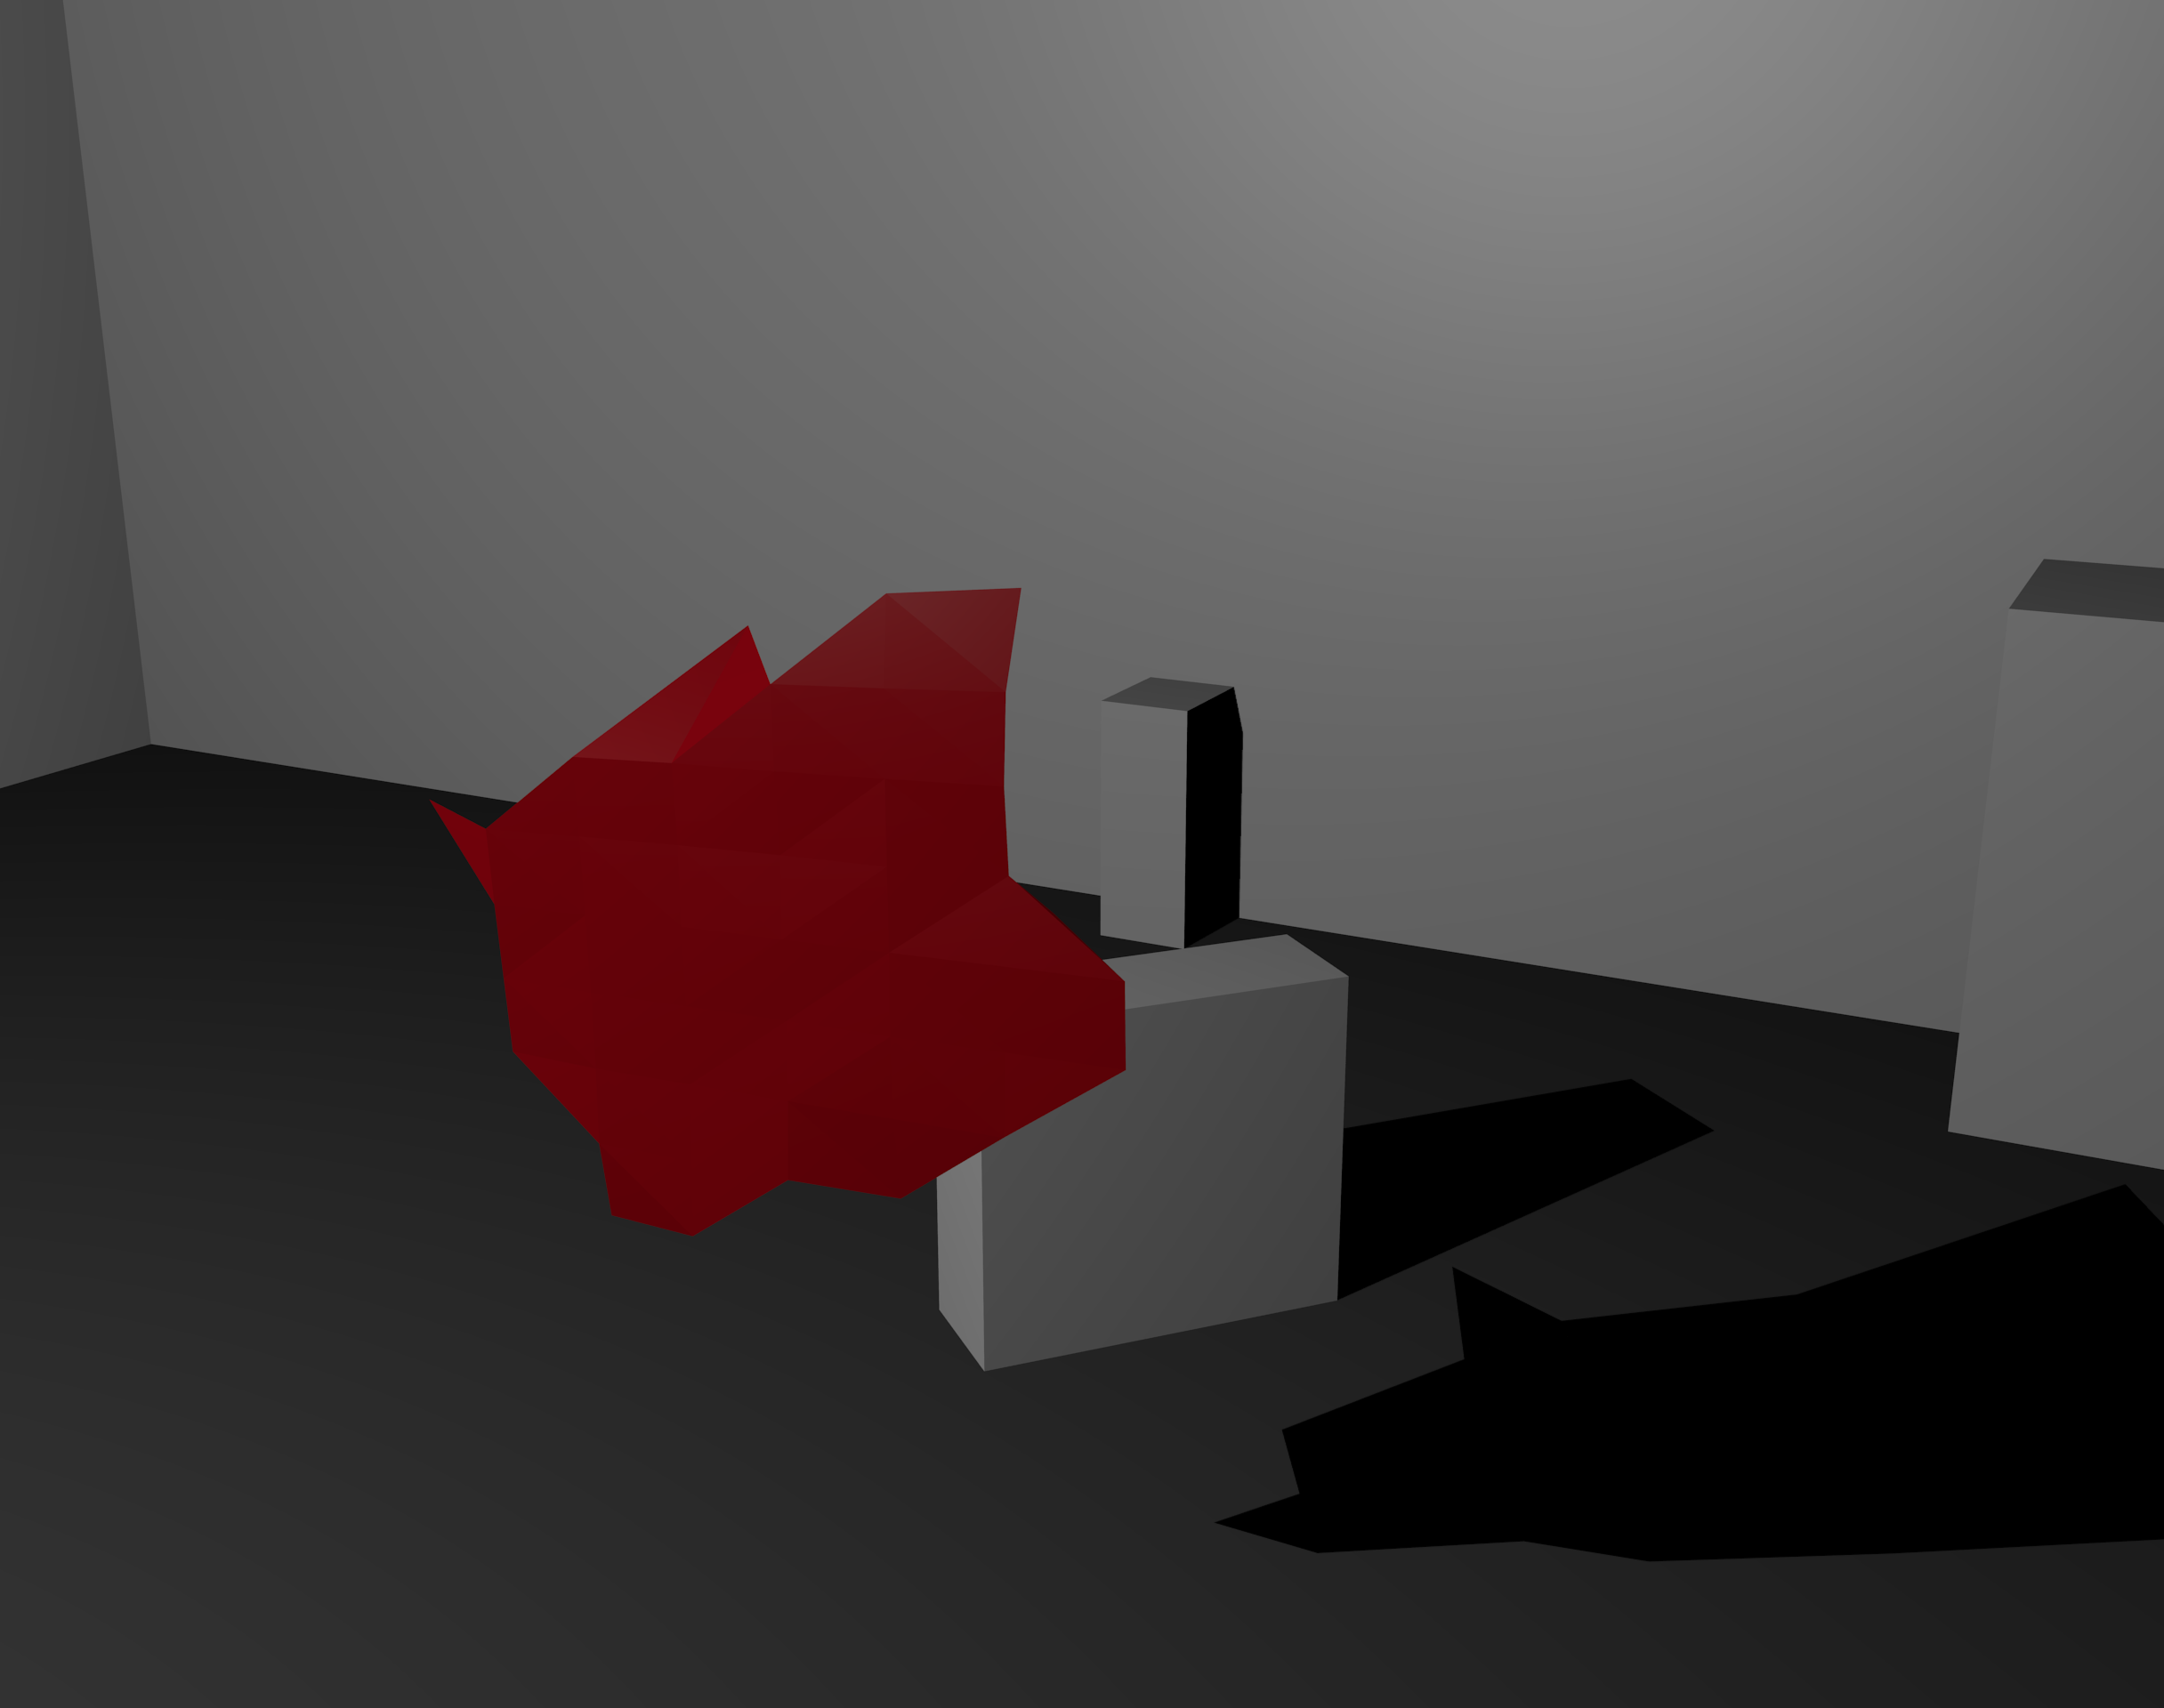
\includegraphics[width=5.5cm]{img/evaluation/test_set/rendered_obstacle}\\
	(c) Anzeigemodus Hindernis & (d) Hindernis Pointcloud als Mesh
	\end{tabular}
	\caption{Abbildungen (a) - (c) zeigen die sichtbaren Bilder während der Testaufnahme. (d) als Mesh gerenderte Pointcloud}
	\label{fig:test_viewing}
\end{figure}


\subsubsection{\emph{Subimage Detection}}
\label{sec:evaluierung_subimage}

\noindent
\textbf{Großes Hindernis:}\\ 
\noindent
Im ersten Test wurde Hindernis 1 gewählt, dabei wurde mithilfe der dargestellten Hindernisse auf der Disparitätenkarte visualisiert ob sich die Testhindernisse innerhalb des Gefahrenbereichs befinden. Um zu testen, inwieweit sich die Hinderniserkennung auf den tatsächlich definierten Bereich vor dem Kamerasystem beschränkt, wurde das Hindernis zudem zu Teilen außerhalb dieser platziert. Aus den 12 aufgenommenen Bildern des Testsets ergaben sich die in Abbildung \ref{fig:eval_big} (a) sichtbaren Ergebnisse.\\

\begin{figure}[h]
	\centering
	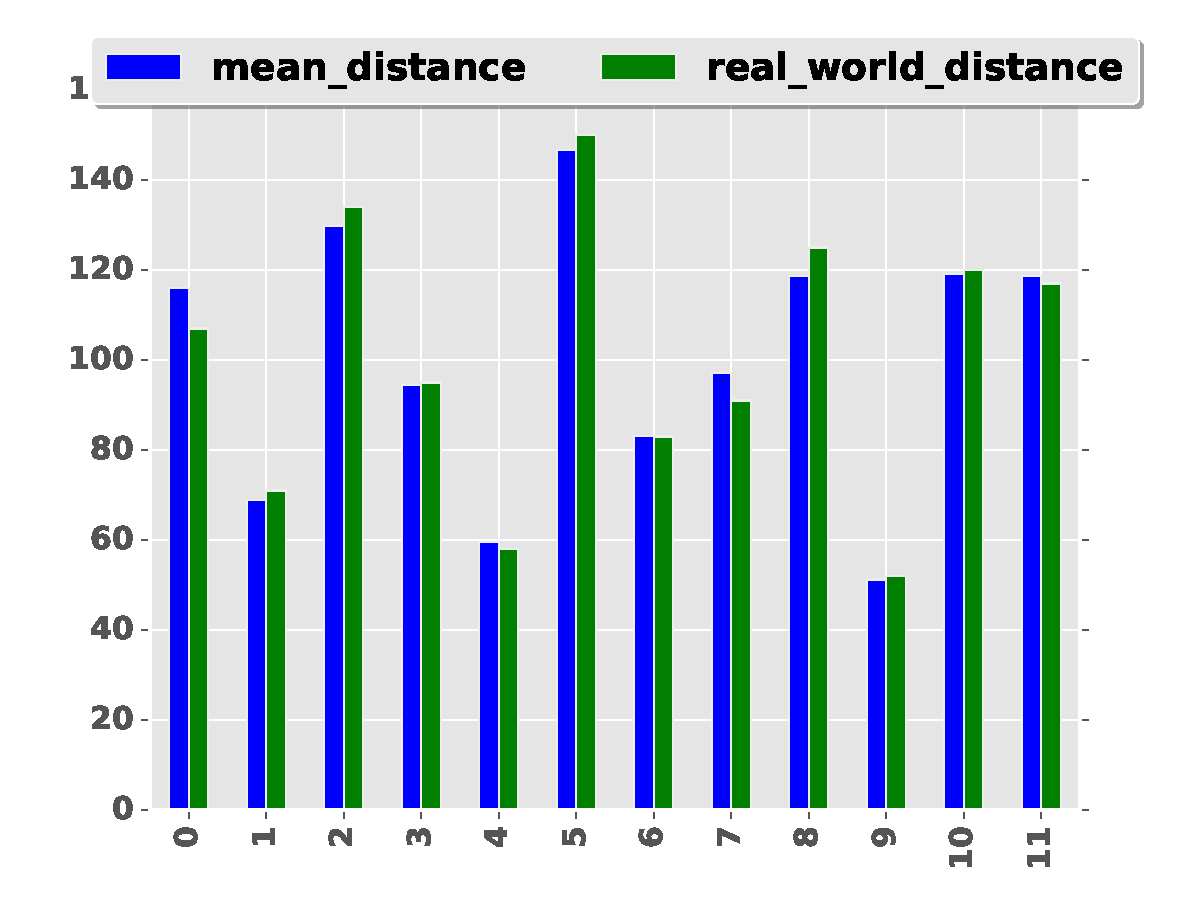
\includegraphics[width=8.5cm]{img/evaluation/diagrams/sub_big_bar}
	\caption{Abweichung zwischen real gemessener und berechneter Distanz bei Hindernis 1 der \emph{Subimage Detection}}
    \label{fig:eval_big}
\end{figure}

\noindent
Wie aus diesen zu erkennen wurde in nahezu allen Frames das Hindernis richtig erkannt. Die berechneten Distanzen stimmen mit den real gemessenen überein. Minimale Abweichungen im Bereich von 2-6 Zentimetern können in diesem Fall als Messungenauigkeit ignoriert werden, da der Mittelpunkt zwischen der minimalen und maximalen Objektdistanz nicht genau bestimmbar war und die Streckenmessung mittels Laser-Entfernungsmesser oder Maßband aufgrund der fehlenden Information über die genaue Lage des Projektionszentrums der Referenzkamera nicht genauer als die mittlere Abweichung ist. Die durchschnittliche Abweichung von berechneten zu real gemessenen Werten betrug dabei $0,02$ Zentimeter. Die Standardabweichung der Differenzen beträgt $4,0$ Zentimeter. Dies deutet auf eine allgemein robuste Erkennung von Hindernis 1 durch die \emph{Subimage Detection} hin.

\pagebreak
\noindent
\textbf{Mittleres Hindernis:}\\
\begin{figure}[h]
	\centering
	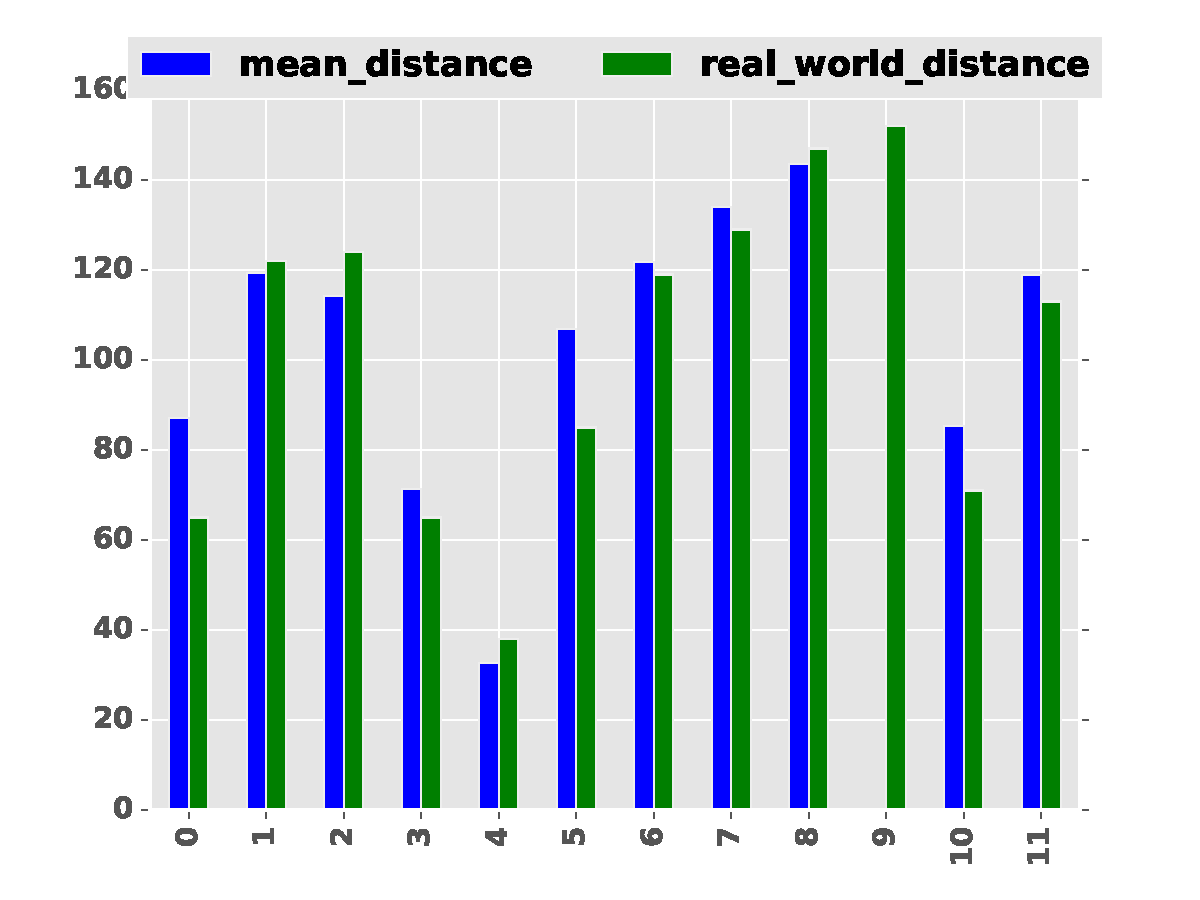
\includegraphics[width=8.5cm]{img/evaluation/diagrams/sub_medium_bar}
	\caption{Abweichung zwischen real gemessener und berechneter Distanz bei Hindernis 2 der \emph{Subimage Detection}.}
    \label{fig:eval_medium}
\end{figure}

\noindent
Auch die Erkennung mittlerer Hindernisse durch die Methode war in nahezu allen Fällen erfolgreich. Ein auffälliges Detail im Vergleich zu den Ergebnissen des großen Hindernisses ist die höhere Differenz aus berechneter und gemessener Distanz. Auch die durchschnittliche Abweichung von $7,9$ Zentimetern deutet auf eine schlechtere Erkennung der Hindernisse hin. Selbiges lässt sich aus der hohen Standardabweichung von $44,5$ Zentimetern erkennen. Das getestete Objekt befand sich während der Tests an einem durchsichtigen Plexiglas Stab welcher teilweise auch als Hindernis erkannt wurde.\\

\noindent
\textbf{Kleines Hindernis:}\\
\noindent
Die Erkennung von Hindernis 3 durch die \emph{Subimage Detection	} erwies sich als am schlechtesten. In vier von 12 durchgeführten Versuchen wurde das Hindernis nicht mehr erkannt. Auch die restlichen erkannten Hindernisse weisen jeweils eine sehr hohe Differenz zwischen berechneter und gemessener Distanz auf (siehe Abbildung \ref{fig:eval_tiny}). Betrachtet man die durchschnittliche Abweichung beider gemessener Distanzen beträgt diese $2,0$ cm. Dies deutet zunächst auf keine besonders schlechte Erkennung hin. Die Standardabweichung von $63,9$ Zentimetern zeigt jedoch die hohe Fehlerrate der Methode bei Hindernis 3.

\begin{figure}[h]
	\centering
	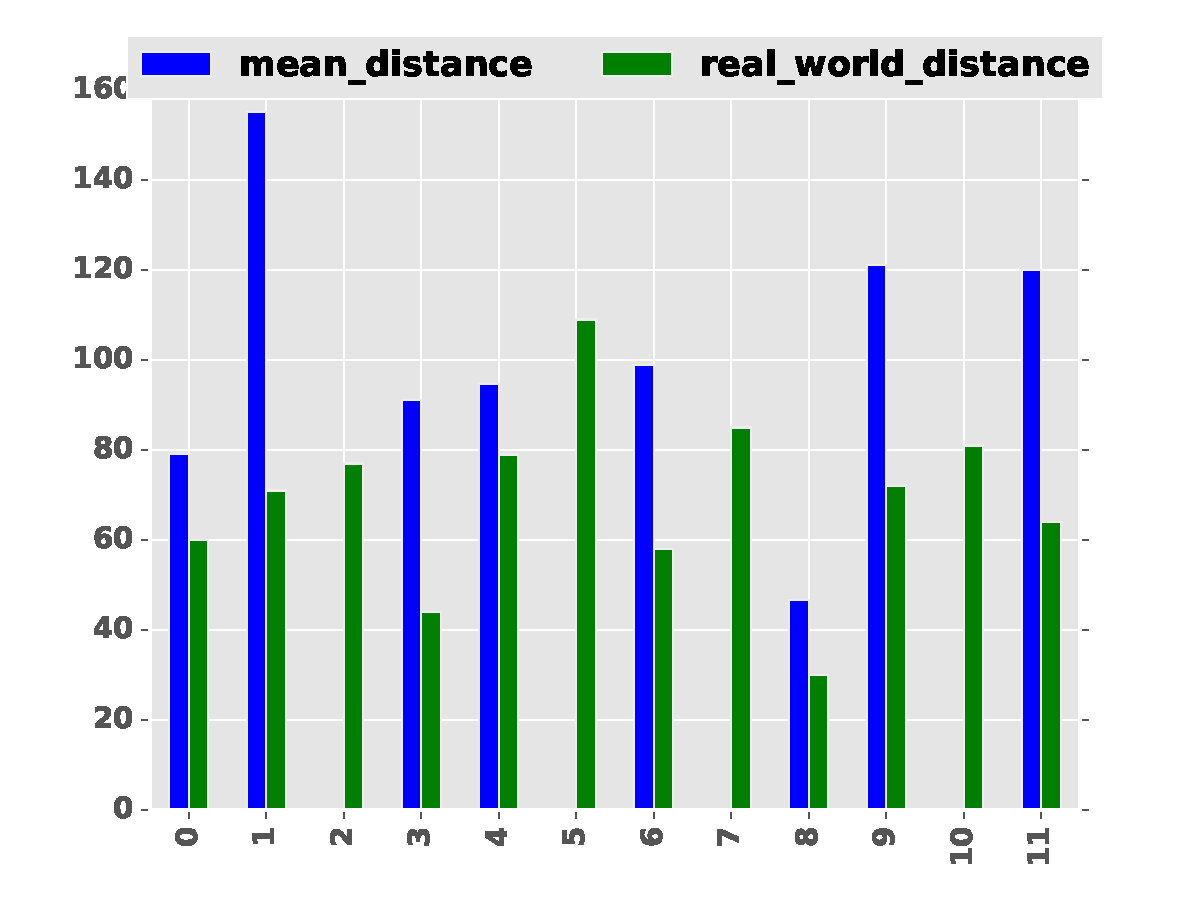
\includegraphics[width=8.5cm]{img/evaluation/diagrams/sub_tiny_bar}
	\caption{Abweichung zwischen real gemessener und berechneter Distanz bei Hindernis 3 der \emph{Subimage Detection}.}
    \label{fig:eval_tiny}
\end{figure}


%%%%%%%%%%%%%%%%%%%%%%%%%%%%%%%%%%%%%%%%%%%%%%%%%%%%%%%%%
% ---------------------- SECTION ---------------------- %
%%%%%%%%%%%%%%%%%%%%%%%%%%%%%%%%%%%%%%%%%%%%%%%%%%%%%%%%%
\pagebreak
\subsubsection{\emph{Samplepoint Detection}}
\label{sec:evaluierung_samplepoint}

\noindent
Im Rahmen dieses Abschnittes wird die \emph{Samplepoint Detection} getestet. Durch die wesentlich höhere Anzahl an betrachteten Bereichen innerhalb der Disparitätenkarte ist anzunehmen, dass die Erkennung kleiner Hindernisse mit diesem Verfahren eine höhere Erfolgswahrscheinlichkeit verspricht. Dies geschieht nach dem in \ref{sec:evaluierung_subimage} bereits beschriebenen Schema. Zur Initialisierung der Methode wurde der Radius der \emph{Samplepoints} auf 2 Pixel gesetzt, was einer Gesamtanzahl von 25 Pixeln pro \emph{Samplepoint} entspricht.\\

\noindent
\textbf{Großes Hindernis:}\\
Die Erkennung großer Objekte der \emph{Samplepoint Detection} weist nahezu keine Fehler auf. Abbildung \ref{fig:sample_eval_big} zeigt das jede der 12 Ausrichtungen des Objektes erkannt wurden. Die dabei auftretenden Differenzen zwischen der berechneten sowie gemessenen Distanz sind auf Messungenauigkeiten, durch die Verwendung des Maßbandes sowie Laser-Entfernungsmessers, zurückzuführen. Auch in Grenzbereichen nahe dem Rand des Gefahrenbereichs wurden die Hindernisse erkannt. Mittlere Differenz sowie die Standardabweichung zwischen der gemessenen sowie berechneten Distanz liegen ebenfalls bei einem Wert von $2,5$ beziehungsweise $2,7$ Zentimetern.\\

\begin{figure}[h]
	\centering
	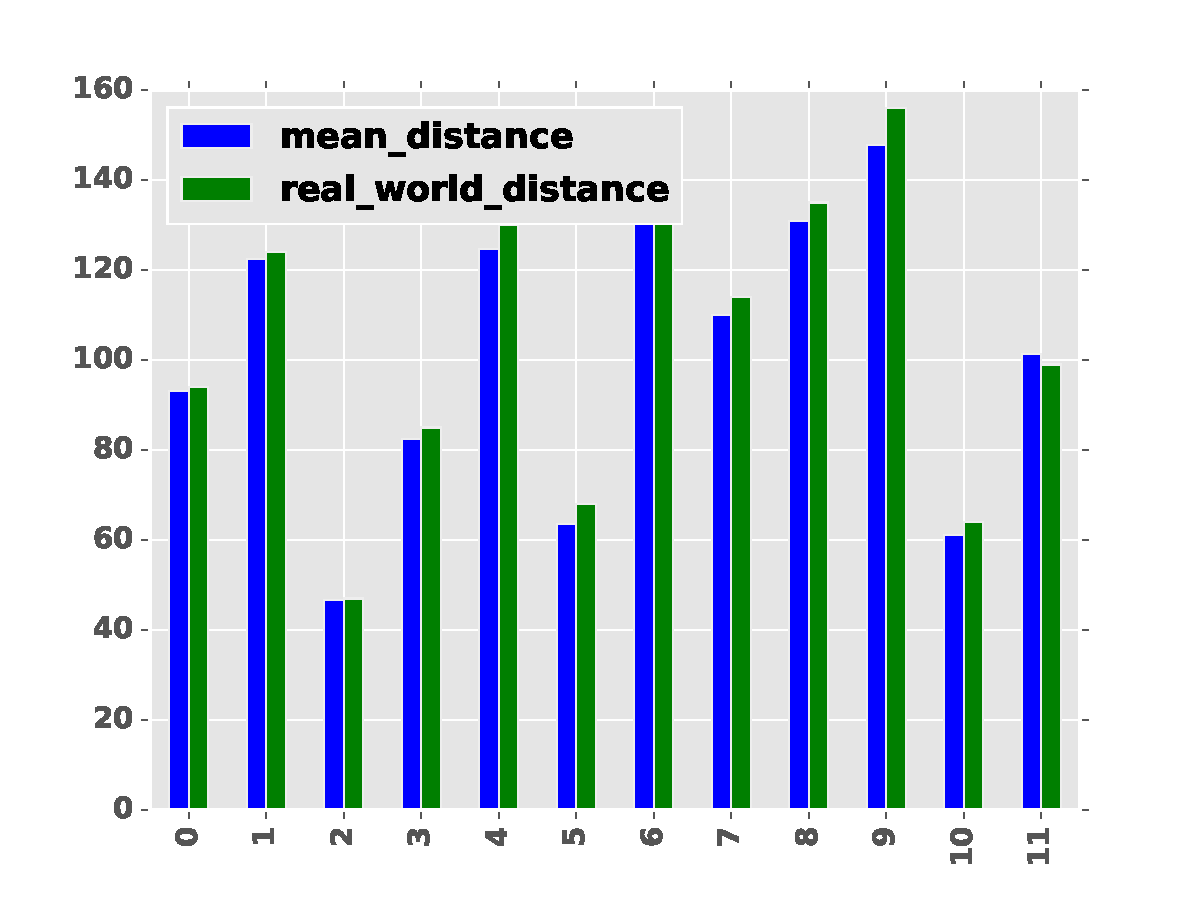
\includegraphics[width=8.5cm]{img/evaluation/diagrams/sample_big_bar}
	\caption{Abweichung zwischen real gemessener und berechneter Distanz bei Hindernis 1 der \emph{Samplepoint Detection}.}
    \label{fig:sample_eval_big}
\end{figure}

\pagebreak
\noindent
\textbf{Mittleres Hindernis:}

\begin{figure}[h]
	\centering
	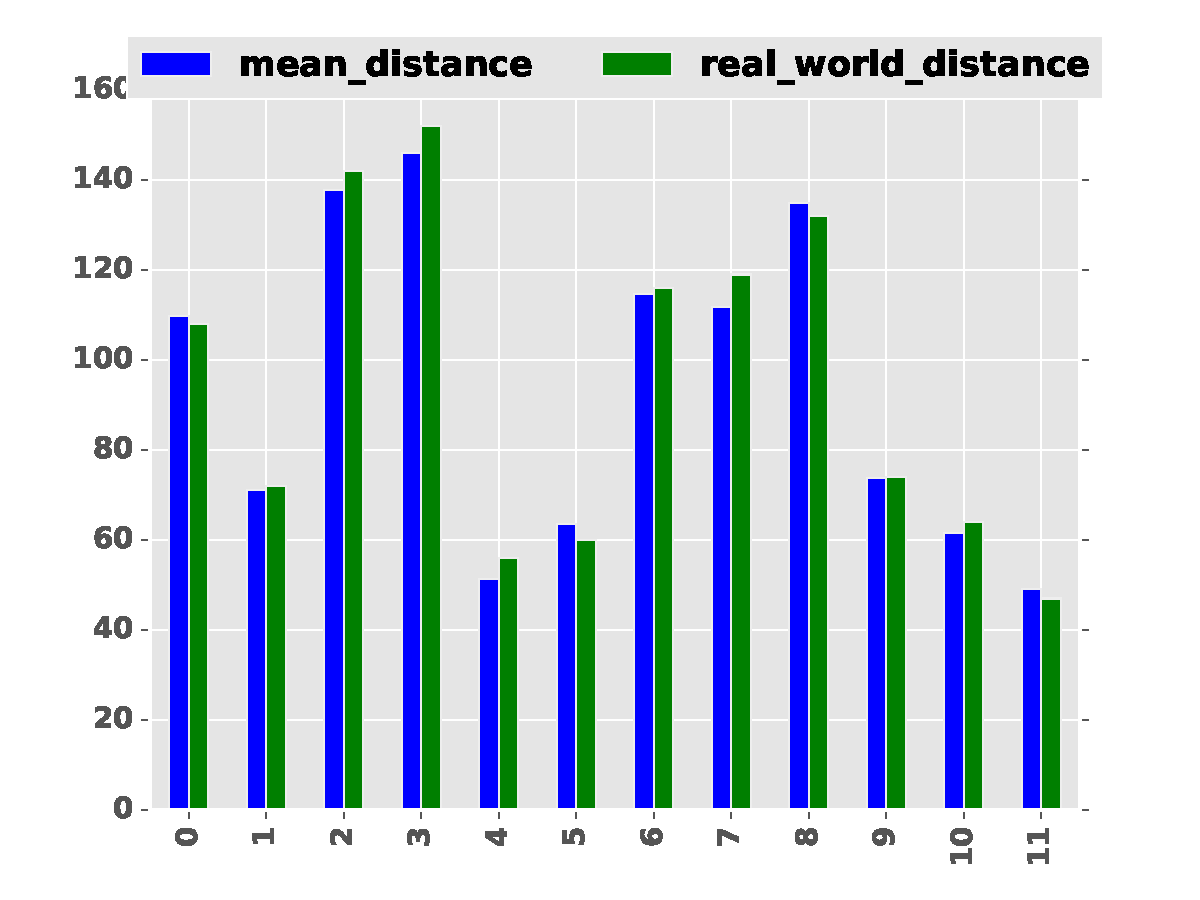
\includegraphics[width=8.5cm]{img/evaluation/diagrams/sample_medium_bar}
	\caption{Abweichung zwischen real gemessener und berechneter Distanz bei Hindernis 2 der \emph{Samplepoint Detection}.}
    \label{fig:sample_eval_medium}
\end{figure}

\noindent
Auch die Erkennung mittlerer Hindernisse erfolgte in allen Frames ohne signifikante Probleme (siehe Abbildung \ref{fig:sample_eval_medium}). Standardabweichung sowie Mittelwert der Differenzen ($1,4$ und $3,4$ Zentimeter) belegen auch hier die sehr gute Erkennung der einzelnen Hindernisse.\\

\pagebreak
\noindent
\textbf{Kleines Hindernis:}\\
Die anfangs aufgestellte These, dass sich die Verteilung sowie Größe der \emph{Samplepoints} positiv auf die Erkennung diverser Hindernisse auswirkt wird mit den Ergebnissen des kleinen Hindernisses bestätigt. Abbildung \ref{fig:sample_eval_tiny} belegt diese Aussage. Es wurden alle 12 Hindernisse ohne signifikant hohe Differenz zwischen berechneten und gemessenen Distanzen erkannt.

\begin{figure}[h]
	\centering
	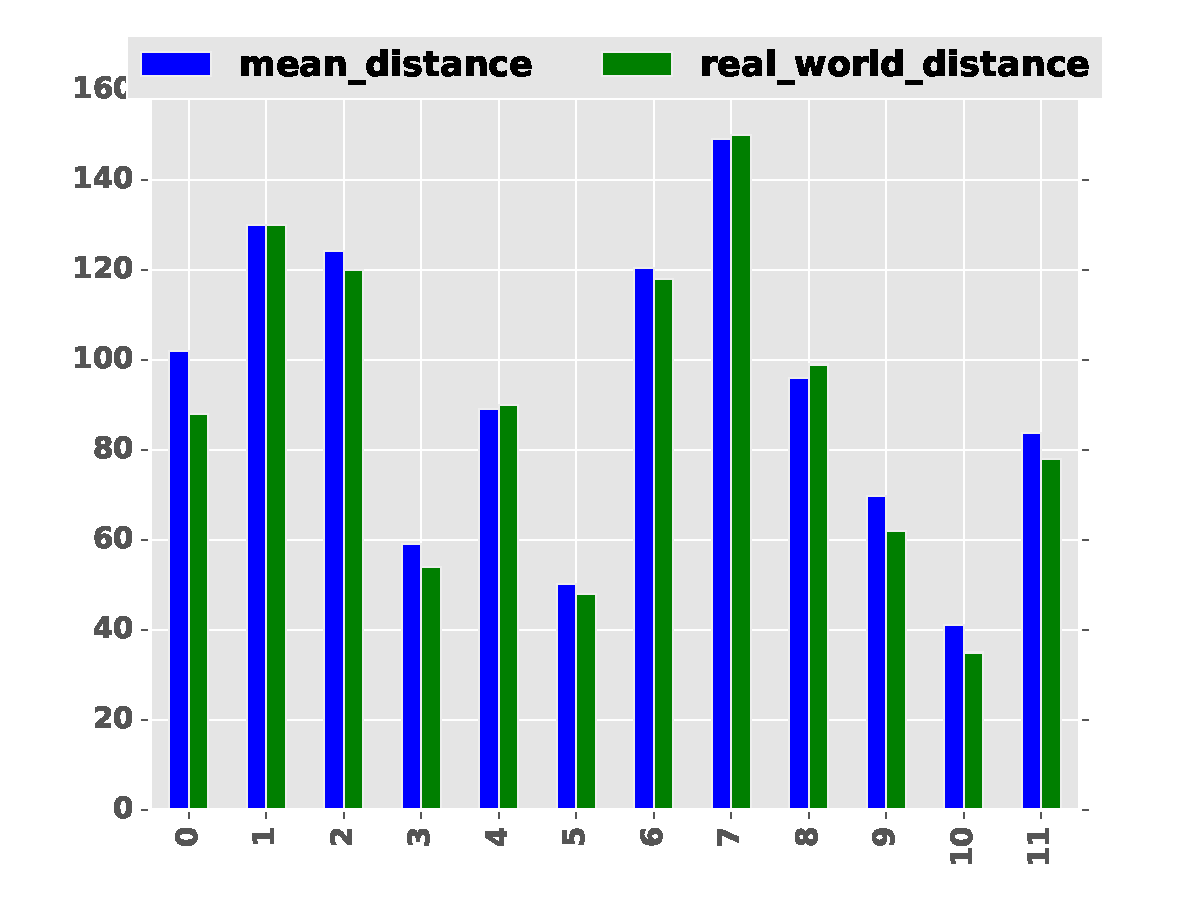
\includegraphics[width=8.5cm]{img/evaluation/diagrams/sample_tiny_bar}
	\caption{Abweichung zwischen real gemessener und berechneter Distanz bei Hindernis 3 der \emph{Subimage Detection}.}
    \label{fig:sample_eval_tiny}
\end{figure}

\noindent
Weiterhin ist auch die statistische Auswertung der Differenzen ein Zeichen für die robuste Erkennung kleiner Hindernisse. Die mittlere Differenz zwischen berechneten und gemessene Werten beträgt lediglich $3,5$ Zentimeter. Auch die Standardabweichung von $4,5$ cm deutet auf eine sehr robuste Erkennung von kleinen Hindernissen hin.

%%%%%%%%%%%%%%%%%%%%%%%%%%%%%%%%%%%%%%%%%%%%%%%%%%%%%%%%%
% ---------------------- SECTION ---------------------- %
%%%%%%%%%%%%%%%%%%%%%%%%%%%%%%%%%%%%%%%%%%%%%%%%%%%%%%%%%
\subsection{Weitere Versuche}
\label{sec:further_tests}

Hinsichtlich der verschiedenen möglichen Faktoren welche eine erfolgreiche Erkennung beeinflussen können wurden im Rahmen der Evaluation beider Algorithmen weitere Tests durchgeführt. Jene umfassen die Erkennung kleiner Hindernisse unter Veränderung der Größe des Matching-Blocks. Weiterhin wird die Erkennung von \enquote{schwierigen} Hindernissen (durchsichtige und  reflektierende Flächen) getestet. Anschließend erfolgt ein weiterer Versuch welcher auf die Veränderung des \emph{Samplepoint} Radius und die damit verbundenen Änderungen in der Erkennung abzielt. Das während der Tests genutzte Setup wurde während der Aufnahme nicht verändert. Auch das Objekt befand sich für jede Blockgröße an der selben Position. Zur Durchführung der Tests wurde das in Abschnitt \ref{sec:evaluierung_subimage} und \ref{sec:evaluierung_samplepoint} genutzte kleine Hindernis verwendet. Auf eine Durchführung der Parameteränderung unter Benutzung des mittleren sowie großen Hindernisses wurde aufgrund der robusten Ergebnisse beider bewusst verzichtet.\\

\noindent
\subsubsection{Einfluss der \emph{SGBM} Block Größe}
\label{subsec:block_size_change}

\textbf{Subimage Detection:}\\
\noindent
Um die Auswirkungen der Blockgröße auf die Distanzberechnung zu testen wurden verschiedene Kantenlängen des Blocks getestet. Für jede Größe wurde die Hinderniserkennung aus je 3 Distanzen ausgeführt. Im Folgenden werden zunächst die Daten dargelegt und im Anschluss daran analysiert. Eine Diskussion der erhaltenen Ergebnisse findet in Abschnitt \ref{sec:evaluation_Diskussion} statt.\\

\begin{table}[h]
\centering
\begin{tabular}{|l||c|c|}
\hline
Blockgröße & berechnete Distanz (cm)& real gemessene Distanz (cm)\\
\hline\hline
7          & 120.6          		& 50                     \\
           &  -                 & 100                    \\
           &  -                 & 150                    \\
\hline
9          & 105.8          		& 50                     \\
           &  -                 & 100                    \\
           &  -                 & 150                    \\
\hline
11         & 98.9           		& 50                     \\
           &  -                 & 100                    \\
           &  -                 & 150                    \\
\hline
13         & 85.2          		& 50                     \\
           &  -                 & 100                    \\
           &  -                 & 150                    \\
\hline
15         & 112.1		        & 50                     \\
           &  -                 & 100                    \\
           &  -                 & 150                    \\
\hline
21         & 108.6         		& 50                     \\
           &  -                 & 100                    \\
           &  -                 & 150                    \\
\hline
\end{tabular}
\caption{Ausgewertete Daten des Subimage Sets}
\label{tbl:distance_subimage}
\end{table}	

\noindent
Wie aus Abbildung \ref{tbl:distance_subimage} ersichtlich wird hat eine Änderung der Blockgröße keine Auswirkungen auf die Erkennung des Objektes. Die Hindernisse wurden lediglich bei einer Distanz von 50 Zentimetern erkannt, wobei die berechneten Werte eine starke positive Abweichung aufweisen. \\

\noindent
\textbf{Samplepoint Detection:}

\begin{table}[h]
\centering
\begin{tabular}{|l||c|c|}
\hline
Blockgröße & berechnete Distanz (cm) & real gemessene Distanz (cm) \\
\hline\hline
7          & 63.8               & 50                     \\
           & 102.2              & 100                    \\
           & 149.1              & 150                    \\
\hline
9          & 57.3               & 50                     \\
           & 107.9              & 100                    \\
           & 153.6              & 150                    \\
\hline
11         & 68.0               & 50                     \\
           & 107.1              & 100                    \\
           & 149.1              & 150                    \\
\hline
13         & 51.4               & 50                     \\
           & 101.4              & 100                    \\
           & 151.1              & 150                    \\
\hline
15         & 57.3               & 50                     \\
           & 105.3              & 100                    \\
           & 149.1              & 150                    \\
\hline
21         & 56.0               & 50                     \\
           & 101.5              & 100                    \\
           & 147.3              & 150                    \\
\hline
\end{tabular}
\caption{Ausgewertete Daten des Subimage Sets }
\label{tbl:distance_samplepoint}
\end{table}

\noindent
Die Änderung der Blockgröße hat auch bei der \emph{Samplepoint Detection} keinen signifikanten Einfluss auf die Erkennung oder Berechnung der Hindernisdistanz. Im Gegensatz zur \emph{Subimage Detection} wurden jedoch alle Distanzen auch korrekt berechnet. Die Differenz zwischen den berechneter und gemessener Distanz ist bei 13 Pixeln Blockgröße am geringsten.


\subsubsection{Erkennung von reflektierenden und durchsichtigen Bereichen}
\label{subsec:test_reflection_translucency}

Die Erkennung von Hindernissen bei reflektierenden sowie durchsichtigen \linebreak Flächen wurde mit drei verschiedenen Tests untersucht. Zunächst wurde untersucht wie sich das System bei spiegelnden Flächen (etwa Fensterglas) verhält. Anschliessend wurde die Erkennung bei reflektierenden Flächen untersucht sowohl im 90$^\circ$ Winkel, also mit direkter Sicht auf das zu erkennende Hindernis als auch unter diversen anderen Winkeln. Weiterhin wurde untersucht inwiefern sich das System bei einer Kombination beider Problemstellungen verhält. Die verwendete Methode zur Hinderniserkennung ist in allen folgenden Tests die \emph{Samplepoint Detection} aufgrund der bisherigen besseren Ergebnisse. Die Gefahrenzone wurde aus Platzgründen auf $0,1$ bis $1,0$ Meter definiert.\\

\noindent
Zur Untersuchung reflektierender Flächen wurde der spiegelnde Bildschirm eines LED-Fernsehers genutzt. Da die Berechnung von Disparitätenkarten auch unter nicht optimalen Lichtverhältnissen robuste Ergebnisse liefert (Abbildung \ref{fig:dark_disparity}) stellt auch die schwarze Grundfarbe des spiegelnden Objektes prinzipiell keinen Konflikt dar. Trotz dessen wurde die Belichtungszeit der Kameras auf 60 - 70 µs gesetzt, was die erhaltenen Bilder in ihrer Helligkeit erheblich verbessert.\\

\begin{figure}[h]
	\centering
	\begin{tabular}{ccc}
		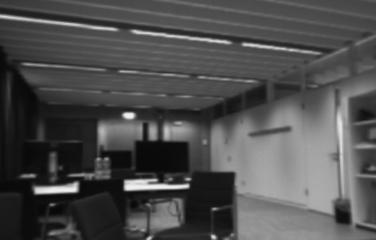
\includegraphics[width=5cm]{img/brightness/bright_left} &
		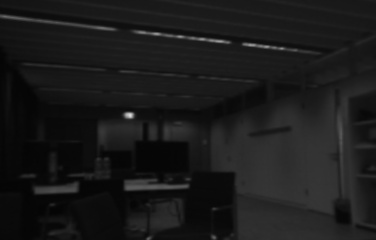
\includegraphics[width=5cm]{img/brightness/middle_left} \\
		(a1) &
		(b1)\\
		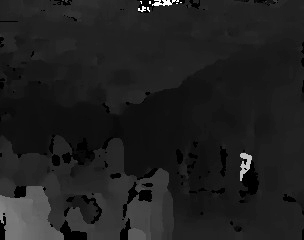
\includegraphics[width=5cm]{img/brightness/bright_dis} &
		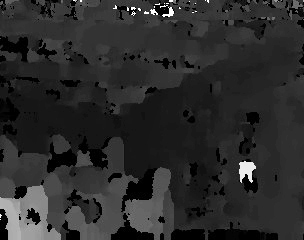
\includegraphics[width=5cm]{img/brightness/middle_dis} \\
		(a2) &
		(b2)
	\end{tabular}
	\caption{Vergleich zwischen einer hellen aufgenommenen Szene in (a1) und (a2) sowie den dazu gehörigen Disparitätenkarten in (a2) und (b2).}
	\label{fig:dark_disparity}
\end{figure}

\noindent
Die aufgenommenen Ergebnisse zeigen auf das Hindernisse erkannt wurden, jedoch ist der Ursprung dieser nicht eindeutig zu erkennen. Abbildung \ref{fig:reflection_only} stellt die berechneten und aufgenommenen Distanzen gegenüber. Aus diesen sind ebenfalls deutlich die Fehler innerhalb der Berechnung zu erkennen.\\

\begin{figure}[h]
	\centering
	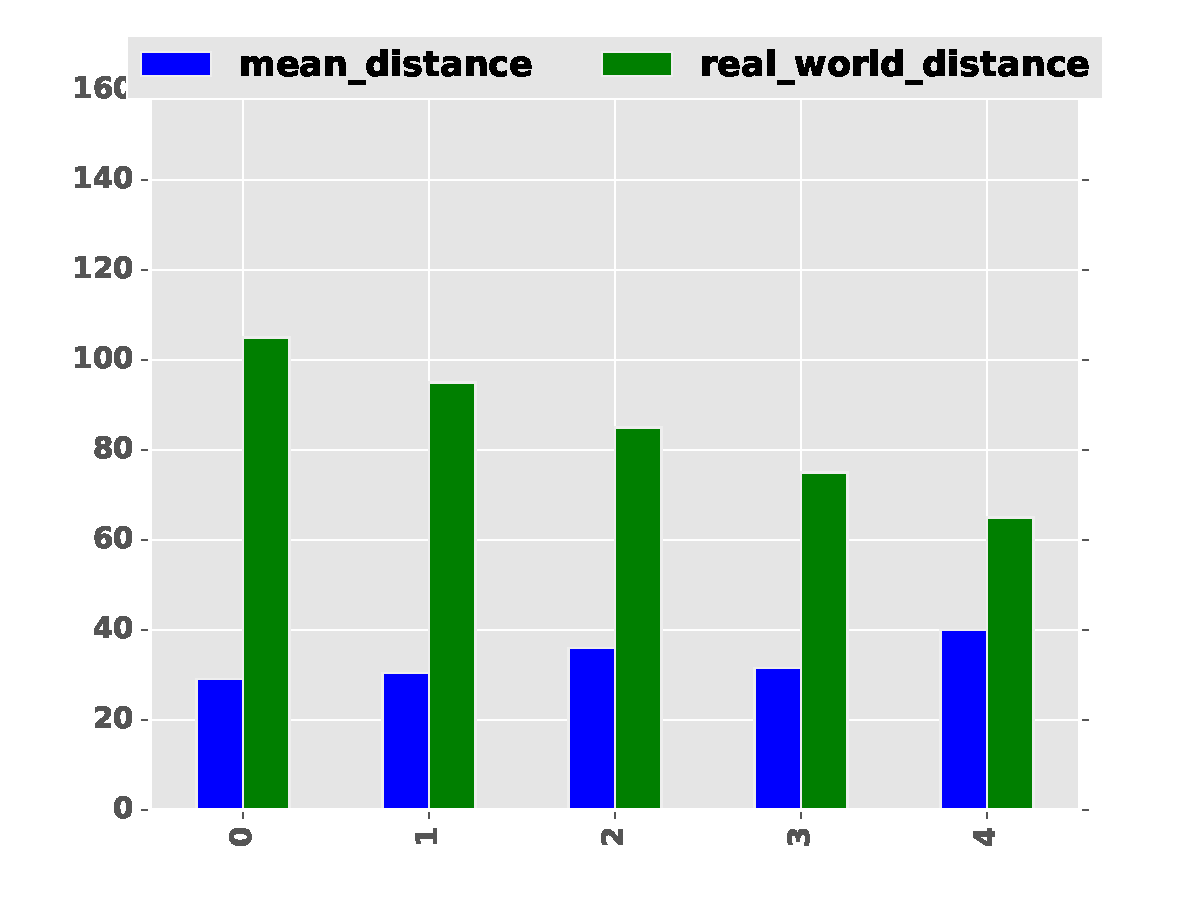
\includegraphics[width=7cm]{img/reflection/reflection_bar}
	\caption{Darstellung Abweichung zwischen real gemessener und berechneter Distanz bei reflektierenden Flächen.}
	\label{fig:reflection_only}	
\end{figure}

\pagebreak
\noindent
Ein weiterer durchgeführter Versuch beinhaltet die Veränderung des Winkels zwischen Kamera und reflektierender Ebene. Die ausgehende Vermutung ist die Erkennung dieser aufgrund diverser Lichtreflexionen. Dazu wurden die Bilder aus 3 verschiedenen Winkeln (45, 22,5 und 12,25$^\circ$) unter Verwendung der Mitte der Basislinie als Rotationszentrum aufgenommen. Dabei repräsentieren die einzelnen Versuche die jeweiligen Winkel in absteigender Reihenfolge. Die gemessenen Distanzen repräsentieren jeweils die Hypotenuse des rechtwinkligen Dreiecks welches durch die Kameras und die beiden Punkte auf der Reflexionsebene gespannt wird. Abbildung \ref{fig:rotation_angle} stellt die erlangten Ergebnisse dar.\\

\begin{figure}[h]
	\centering
	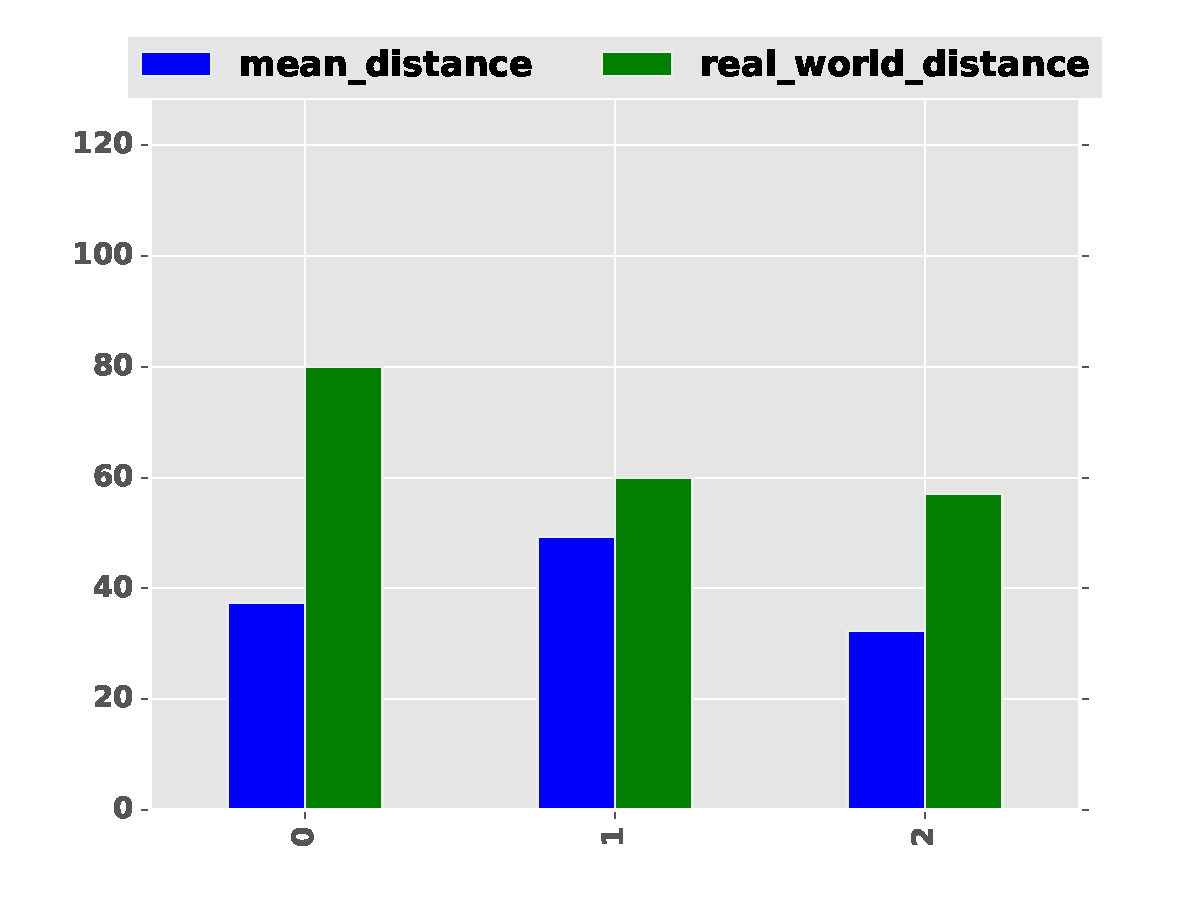
\includegraphics[width=8.5cm]{img/reflection/angle_bar}
	\caption{Abweichung zwischen real gemessener und berechneter Distanz bei reflektierenden Flächen unter Veränderung Aufnahmewinkels zur reflektierenden Fläche.}
	\label{fig:rotation_angle}
\end{figure}

\noindent
Aus diesen wird ersichtlich, dass kein Hindernis valide erkannt werden konnte. Die Differenz zwischen gemessenen und berechneten Distanzen deutet auf Fehler in der Berechnung der Disparitätenkarte aufgrund der Reflexion hin.\\

\noindent
Eine Kombination von Reflexion und Durchsichtigkeit brachte ebenfalls keine validen Ergebnisse. In den ersten fünf Versuchen wurden zwar Hindernisse erkannt, jedoch weitaus näher, als sie sich eigentlich befunden haben. Zudem wurden Hindernisse erkannt obwohl sich keines innerhalb der Gefahrenzone befunden hat. Die somit erkannten Hindernisse wirken demnach als Resultat zufälliger Matches. Ab Versuch 5 befand sich das Fenster innerhalb der Gefahrenzone. Abbildung \ref{fig:combined} zeigt eben diese Ergebnisse.\\

\begin{figure}[h]
	\centering
	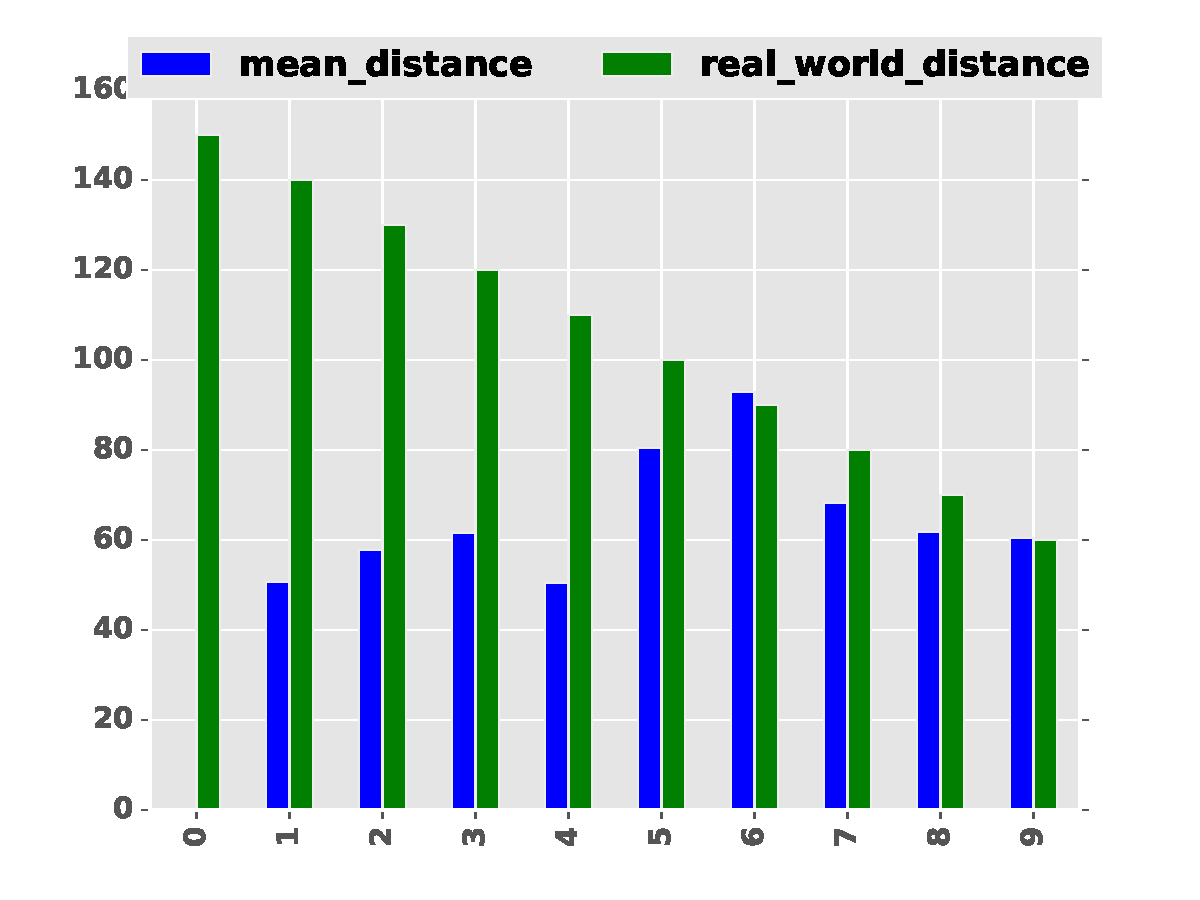
\includegraphics[width=8.5cm]{img/reflection/combined_bar}
	\caption{Abweichung zwischen real gemessener und berechneter Distanz bei reflektierenden einer Kombination von Reflexion sowie Durchsichtigkeit des zu findenden Hindernis}
	\label{fig:combined}
\end{figure}

\subsubsection{Erkennung unter Veränderung des Samplepoint Radius}
\label{subsec:test_samplepoint_radius}

Im Gegensatz zu \emph{Subimages} bietet die Verwendung von \emph{Samplepoints} neben der Gefahrenzone die Größe des Radius als veränderlichen Parameter. Im Rahmen der Evaluierung wurde getestet welche Auswirkung die Modifikation dessen auf die Erkennung hat. Dazu wurden die Konfigurationen 0 - 4 (0 indiziert dabei keinen Radius und somit die Verwendung eines einzelnen Pixels) mit jeweils fünf verschiedenen Positionen des kleinen Hindernisses getestet. Hindernis 1 und 2 wurden aufgrund der vorherigen robusten Ergebnisse in diesem Test nicht betrachtet.\\

\noindent
Die Veränderung des Samplepoint Radius brachte lediglich bei der Verwendung eines einzelnen Pixels eine wahrzunehmende Veränderung mit sich. Das Hindernis wurde bei größeren Entfernungen zwar besser erkannt, jedoch wurden ebenfalls Bereiche mit Fehlinformationen als Hindernis gedeutet. Dies bestätigt die Verwendung der lokalen Nachbarschaft zur Erweiterung des Suchfeldes als wichtiges Kriterium für die Erkennung.

%%%%%%%%%%%%%%%%%%%%%%%%%%%%%%%%%%%%%%%%%%%%%%%%%%%%%%%%%
% ---------------------- SECTION ---------------------- %
%%%%%%%%%%%%%%%%%%%%%%%%%%%%%%%%%%%%%%%%%%%%%%%%%%%%%%%%%
\pagebreak
\section{Diskussion}
\label{sec:evaluation_Diskussion}

Im Rahmen dieses Kapitels wurden beide entwickelten Methoden in verschiedenen Versuchen getestet. Beide Methoden erkennen sowohl große als auch mittlere Hindernisse innerhalb der definierten Gefahrenzone. Die ermittelten Distanzen weisen zwar kleine Ungenauigkeiten auf, jedoch sind diese eher ein Resultat von Messungenauigkeiten sowie der verwendeten Bildgröße. Es erfolg somit eine Auswertung der erlangten Ergebnisse, sowie eine Gegenüberstellung beider Algorithmen in Hinsicht auf die Robustheit der Erkennung sowie deren Laufzeit.

\subsection{Robustheit}
\label{subsec:discussion_robustness}

% FIRST

Die in den Abschnitten \ref{sec:evaluierung_subimage} und \ref{sec:evaluierung_samplepoint} erlangten Ergebnisse belegen die generelle Effektivität und Robustheit beider Algorithmen. Die Grundidee der Methoden gleicht sich in einigen Punkten, ebenso die Resultate. Beide Algorithmen liefern robuste Ergebnisse unter der Voraussetzung einer gewissen Hindernisgröße, wobei das kleine Objekt die größte Anforderung an diese darstellt. Die Detektion des großen sowie mittleren Hindernisses ergab in allen Versuchen die Ergebnisse mit den niedrigsten Differenzen zwischen berechneten und gemessenen Entfernungen.

%%% SUBIMAGE DETECTION
\subsubsection{Subimage Detection}
\noindent
Das Konzept der \emph{Subimage Detection} ist in Bezug auf große und mittlere Hindernisse als robust einzustufen, jedoch ist die Berechnung des Mittelwertes der Matrizen auch der größte Konflikt. Weist der Hintergrund eines Objektes sehr geringe Disparitäten auf, so besteht die Möglichkeit das der Hintergrund den Mittelwert eines einzelnen \emph{Subimages} insofern beeinflusst, dass das Hindernis (innerhalb dieser Submatrix) nicht mehr erkannt werden kann. Dies ließ sich bei nahezu allen Versuchen und Hindernisgrößen beobachten. Im Fall der großen und mittleren Hindernisse stellt dies keinen maßgeblichen Konflikt dar, da die Fläche der Hindernisse trotzdem für eine Erkennung ausreicht. Ungeachtet dessen stellt gerade dieser Konflikt ein Problem in der Erkennung einzelner kleiner Hindernisse dar.\\

% GROSSES HINDERNIS SUBIMAGE
\noindent
Bei der Erkennung großer Hindernisse wurden diese zwar alle erkannt, jedoch nicht der gesamte Bereich den sie umfasst haben. Wie Abbildung \ref{fig:eval_big_fails} zeigt wurden der obere und untere Bereich des Hindernisses im 5. Frame nicht erkannt. Dies resultiert daraus, dass nur ein geringerer Anteil der Pixel dieser Segmente das Objekt repräsentieren, so dass der Mittelwert in diesem Fall maßgeblich durch die sehr kleinen Disparitäten des Hintergrunds verkleinert wird.\\

\begin{figure}[h]
	\centering
	\begin{tabular}{cc}
	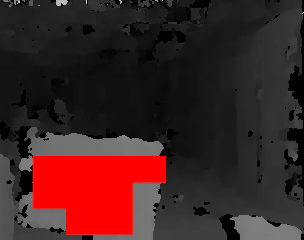
\includegraphics[width=5cm]{img/evaluation/_test_5_disparity}&
	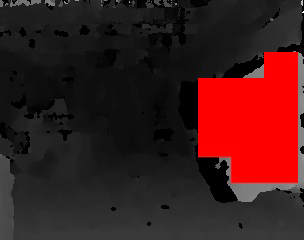
\includegraphics[width=5cm]{img/evaluation/_test_8_disparity}\\
	(a) &  (b)
	\end{tabular}
	\caption{Darstellung des in Versuch 5 (a) und Versuch 8 (b) gefundenen Hindernisse, rot markierte Bereiche zeigen ein erkanntes Hindernis innerhalb eines \emph{Subimages} }
    \label{fig:eval_big_fails}
\end{figure}

%% MITTLERES HIDNERNIS SUBIMAGE
\noindent
Die Detektion von Hindernis 2 gelang ebenfalls in allen Versuchen, jedoch zeigen die Werte eine größere Abweichung in den Differenzen von berechneter und gemessener Distanz. Im Fall von Frame 0 umfasst das Objekt insgesamt 17 \emph{Subimages} in denen es erkannt wurde. Als Resultat des Stabes wurden jedoch noch 2 weitere erkannt. Frame 1 weist zwar keine große Abweichung zwischen der berechneten und realen Distanz auf, jedoch wird das Objekt zu Teilen nicht erkannt. Grund dafür ist wiederum der bereits beschriebene weit entfernte Hintergrund. Bei einer Distanz von 120 Zentimetern ist eine Erkennung dieser Hindernisgröße in nur 2 \emph{Subimages} ungewöhnlich. Dies resultiert aus der verwendeten Blockgröße.\\

\begin{figure}[h]
	\centering
	\begin{tabular}{cc}
	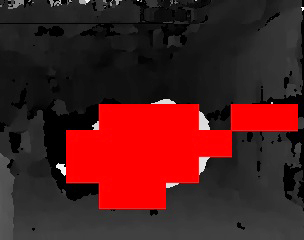
\includegraphics[width=5cm]{img/evaluation/medium_test_0_disparity}&
	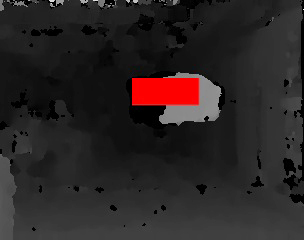
\includegraphics[width=5cm]{img/evaluation/medium_test_1_disparity}\\
	(a) & (b)
	\end{tabular}
	\caption{Darstellung des in Versuch 0 (a) und Versuch 3 (b) gefundenen Hindernisse, rot markierte Bereiche zeigen ein erkanntes Hindernis innerhalb eines \emph{Subimages} }
	\label{fig:eval_medium_fails}
\end{figure}

\noindent
Selbiges Resultat lässt sich in den Frames 2, 6 und 7 erkennen. In Frame 9 dagegen konnte kein Hindernis erkannt werde, da sich das Objekt an der Grenze der Gefahrenzone befunden hat und demnach die Abweichung der Disparität zu keiner Erkennung führen konnte.\\


%% KLEINES HINDERNIS SUBIMAGE
\noindent
Die Erkennung kleiner Hindernisse gestaltet sich aufgrund diverser Faktoren schwer. Ein limitierender Faktor ist die Fläche. Ist ein einzelnes Hindernis so klein, dass es während der Berechnung des Mittelwertes aufgrund der umliegenden Disparitäten untergeht, so kann auch kein Hindernis erkannt werden. Dies macht sich in vielen der getesteten Bildern bemerkbar. In den Frames 2, 5, 7 und 10 wurde das Hindernis nicht erkannt, da es sich entweder an einer Kreuzung verschiedener \emph{Subimages} befand, oder die verwendete Blockgröße nicht ausreicht, dadurch wird der Mittelwert aller Teilmatrizen nicht signifikant beeinflusst. Auch der Stab wurde in den Frames 3, 6 sowie 8 als zusätzliches Hindernis erkannt. Dies ist ein Resultat der relativ geringen Distanz zu den Kameras. Die hohen Entfernungsdifferenzen resultieren in diesen Fällen wiederum aus der großen Entfernung der Hindernisse zum Hintergrund. Grundlegend ist der hohe Anteil an Hintergrundpixeln im Segment ist in nahezu allen Versuchen der beeinflussende Faktor.

\subsubsection{Samplepoint Detection}
%% SAMPLEPOINT DETECTION
\noindent
Die Erkennung von Hindernissen mit Hilfe der \emph{Samplepoints} ist ebenfalls eine robuste Methode. Dabei reicht die Anzahl der umfassenden Pixel eines jeden aus um selbst kleine Hindernisse zu erkennen. Der nicht beachtete Bereich zwischen den \emph{Samplepoints} kann entweder 6, 4, 2 oder keinen Pixel betragen, in Abhängigkeit des verwendeten Radius. Der fest gewählte horizontale und vertikale Abstand der \emph{Samplepoints} (8 Pixel) reicht jedoch nicht immer um das Hindernis zu erkennen. In vielen Fällen wurde das Hindernis nicht mehr direkt erkannt, sondern die Befestigung dessen. Das Problem befindet sich dabei bei der zugrunde liegenden Disparitätenkarte. Der hintere Bereich der Szene unterscheidet sich farblich nicht signifikant vor der Farbe des Hindernisses. Zudem ist das Objekt bei einer Entfernung von 150 Zentimetern so klein das es höchstwahrscheinlich durch die verwendete Blockgröße nicht erkannt oder mit benachbarten Bereichen verbunden wird.\\

\noindent
Hindernis 1 wurde in allen Versuchen robust erkannt. Die auftretenden Differenzen waren marginal und daher eher Resultat von Messungenauigkeiten. Bereiche in denen aufgrund fehlender Textur keine Korrespondenz zugeordnet werden konnte wurden aufgrund der hohen Dichte der \emph{Samplepoints} trotzdem erkannt. Wie Abbildungen \ref{fig:sample_eval_medium_fails} (a) und (b) zeigen wurden nicht gematchte Bereiche auch nicht als Hindernis erkannt, die umliegenden texturierten Bereiche überwiegen jedoch und sorgen daher für eine Detektion.

\begin{figure}[h]
	\centering
	\begin{tabular}{cc}
	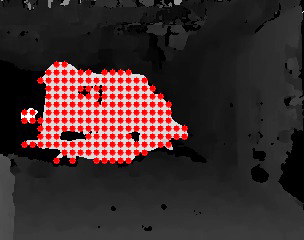
\includegraphics[width=5cm]{img/evaluation/sample_tiny_test_5_disparity} & 
	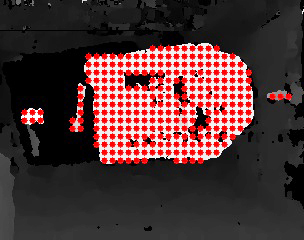
\includegraphics[width=5cm]{img/evaluation/sample_tiny_test_11_disparity}\\
	(a) Frame 5 &  (b) Frame 11
	\end{tabular}
	\caption{Darstellung erkannter Bereiche von Hindernis 2 der \emph{Samplepoint} Detection in Versuch 5 (a) und 11(b) }
	\label{fig:sample_eval_medium_fails}
\end{figure}

%% SAMPLEPOINT KLEINES HINDERNIS
\noindent
Hindernis 3 wurde von der \emph{Samplepoint Detection} ebenfalls überraschend gut erkannt. Trotz dessen ist die Detektion dieser bei Entfernungen von mehr als 60 Zentimetern stark von der Orientierung des Objektes, dem Hintergrund sowie den verwendeten Parametern zur Berechnung der Disparitätenkarte abhängig. Da die geringe Auflösung der Kameras keine detaillierte Aufnahme der Textur des Hindernisses zulässt ist es möglich das das Objekt aufgrund der Blockgröße des \emph{SGBM} mit dem Hintergrund zusammen gematcht wird. 


%%% SGBM BLOCKGROESSE
\subsection{Einfluss der SGBM Blockgröße}
\noindent
Eine Veränderung der SGBM Blockgröße brachte keine signifikanten Verbesserungen in der Hinderniserkennung mit sich. Im Fall der \emph{Subimage Detection} wurden kleine Hindernisse weder besser noch schlechter erkannt. Ab einer Distanz von mehr als 50 Zentimetern erfolgte keine Detektion. Auch die Ergebnisse der \emph{Samplepoint Detection} veränderten sich nicht maßgeblich im direkten Vergleich zur vorherigen Erkennung des kleinen Hindernisses.\\ 

\noindent
Bei den Ergebnissen der \emph{Subimage Detection} werden die berechneten Distanzen erheblich von den Pixeln des Hintergrundes beeinflusst, was in den verzerrten berechneten Distanzen resultiert. Dabei auftretende Differenzen zwischen den real gemessenen Entfernungen sowie den berechneten resultieren aus Interferenzen während der Neuberechnung der Disparitätenkarte in jedem Frame.\\

\noindent
In allen durchgeführten Tests der \emph{Samplepoint Detection} lässt ab einem Abstand von 100 Zentimetern erkennen, dass das eigentliche Hindernis nicht mehr gefunden wurde, sondern die Befestigung dessen das erkannte Hindernis repräsentiert (siehe Abbildung \ref{fig:distance_sample_images}). Ein Grund für diese \enquote{falsch}-Erkennung könnte auch hier die Verwendung des Mittelwertes, sowie der nicht beachtete Raum zwischen den einzelnen Samplepoints sein. Bei einem Radius von 2 Pixeln beträgt dieser ebenfalls 2 Pixel. Eine Verzerrung der Werte durch den Hintergrund ist in diesem Fall unwahrscheinlich, die Verbindung der Distanz sowie der geringen Aufnahmeauflösung der Kameras führt eher dazu, dass das Hindernis vor dem Hintergrund als Teil dessen wirkt. Die plausibelste Fehlerquelle ist daher am wahrscheinlichsten die zugrunde liegende Disparitätenkarte.

\begin{figure}[h]
	\centering
	\begin{tabular}{ccc}
	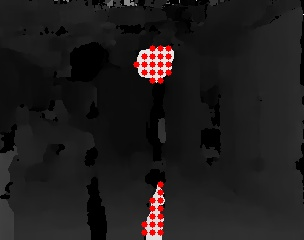
\includegraphics[width=4cm]{img/evaluation/distance_sample/_test_0_disparity}&
	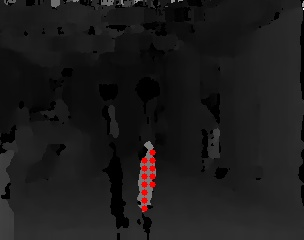
\includegraphics[width=4cm]{img/evaluation/distance_sample/_test_1_disparity}&
	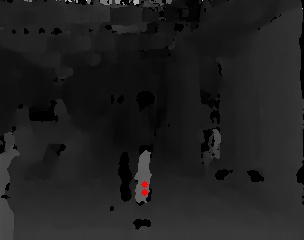
\includegraphics[width=4cm]{img/evaluation/distance_sample/_test_2_disparity}
	\end{tabular}
	\caption{Testset unter Verwendung einer Blockgröße von 13 Pixeln in verschiedenen Distanzen (50 cm bis 150 cm v.l.n.r.)}
	\label{fig:distance_sample_images}
\end{figure}


%%% REFLEKTIERENDE & DURCHSICHTIGE FLAECHEN
\subsection{Erkennung von reflektierenden und durchsichtigen Flächen}
\label{subsec:reflection_discussion}

\noindent
Die Erkennung reflektierender und durchsichtiger Flächen zeigte sich als grundlegend problematisch. Es wurden in nahezu jedem Versuch Hindernisse erkannt, jedoch nur in seltenen Fällen korrekt. Dies kann aus der homogenen Farbgebung der verwendeten Bilder resultieren. Der genaue Ursprung der erkannten Hindernispunkte ist nahezu unmöglich zu identifizieren, da die berechnete Disparitätenkarte keine genaue Lokalisierung von Formen der Szene zulässt. Dies lies sich sowohl bei rein spiegelnden Flächen im 90$^\circ$ Winkel, als auch bei einer Veränderung des Aufnahmewinkels feststellen. Bei einer Kombination von reflektierenden und spiegelnden Flächen wurden zumeist nur wenige Punkte erkannt welche nicht das Objekt als ganzes abbilden (siehe Abbildung \ref{fig:combination_images}). Die gefundenen Hindernisse sind das Resultat eines reflektierten Lichtpunktes auf dem Glas. 

\begin{figure}[!h]
	\centering
	\begin{tabular}{cc}
		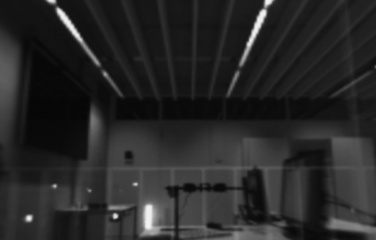
\includegraphics[height=4cm]{img/reflection/reflection_trans_left} &
		
\includegraphics[height=4cm]{img/reflection/reflection_trans_disp} \\
		(a) & (b)
	\end{tabular}
	\caption{Kombination von spiegelnden und durchsichtigen Flächen (a) linkes Referenzbild (b) Berechnete Disparitätenkarte mit markierten Hindernissen}
	\label{fig:combination_images}
\end{figure}

\subsection{Erkennung unter Veränderung des \emph{Samplepoint }Radius}
\label{subsec:radius_change_discussion}
%%%% SUBIMAGE RADIUS
\noindent
Die Anpassung des \emph{Subimage} Radius brachte ebenfalls keine signifikanten Verbesserungen in der Erkennung. Bei einem Radius von 0, also der Verwendung eines einzelnen Pixels wurde Hindernis 3 bei größeren Entfernungen zwar besser erkannt, im gleichen Zug aber auch Ausreißer der Disparitätenkarte. Dieser ungewünschte Nebeneffekt kann bei einer realen Anwendung zu Falschentscheidungen von Seiten der Hindernisvermeidung führen und somit im schlimmsten Fall zum Ausfall des UAS. 

% SECOND
%%% GENERELLER SHIT

%%%%%%%%%%%%%%%%%%%%%%%%%%%%%%%%%%%%%%%%%%%%%%%%%%%%%%%%%
% ------------------- SUBSECTION ---------------------- %

\subsection{Laufzeit}
\label{subsec:discussion_performance}

Hinsichtlich der Performance der entwickelten Systeme wurden verschiedene Punkte betrachtet. Die zugrunde liegende Berechnung der Disparitätenkarte ist der wohl wichtigste Faktor. Ist dieser Prozess langsam, so ist auch die Performance der Hinderniserkennung eingeschränkt. Weiterhin wird auch die Performance der einzelnen Methoden untersucht. Dabei werden folgende Situationen untersucht:
\begin{enumerate}
	\item Analyse der gesamten Schleife des Hauptprogramms
	\begin{enumerate}
		\item Hindernisse bewegen sich durch die Gefahrenzone
		\item der gesamte Sichtbereich ist mit einem Hindernis gefüllt
		\item es befindet sich kein Hindernis in der Gefahrenzone
	\end{enumerate}
	\item Analyse einzelner Erkennungssschritte
	\begin{enumerate}
		\item Geschwindigkeit der \emph{update} Funktion
		\item Geschwindigkeit der \emph{detectObstacles} Funktion mit einem Hindernis im gesamten Sichtbereich
		\item Geschwindigkeit der \emph{detectObstacles} Funktion ohne Hindernisse
	\end{enumerate}
\end{enumerate}

\noindent
Zu Beginn ist ein essenzieller Schritt die Geschwindigkeit der Berechnung der Disparitätenkarte zu analysieren. Dabei wurden beide Kameras im gebinnten Modus getestet. Die Aufnahmerate der Kameras beträgt dabei je nach gewählter Belichtungszeit 55 - 60 Frames pro Sekunde. Die unter Veränderung der Blockgröße erhaltenen Parameter sind in Tabelle \ref{tbl:disparity_framerate} dargestellt. Aus dieser ist zu erkennen, dass eine Modifikation dieses Parameters nur marginale Änderungen in der Geschwindigkeit auftreten. Die folgenden gemessenen Werte sind die durchschnittliche Framerate aus 1000 Einzelbildern.

\begin{table}[h]
	\centering
	\begin{tabular}{|l|c|c|}
	\hline
	Block Größe (Pixel) & Zeit pro Frame (s) & Frames pro Sekunde \\ \hline
	7           & 0.0412         & 24.21              \\ \hline
	9           & 0.0420         & 23.77              \\ \hline
	11          & 0.0413         & 24.17              \\ \hline
	13          & 0.0410         & 24.36              \\ \hline
	15          & 0.0412         & 24.22              \\ \hline
	21          & 0.0413         & 24.17              \\ \hline
	\end{tabular}
	\caption{Blockgröße und daraus resultierende Frameraten}
	\label{tbl:disparity_framerate}
\end{table}

\noindent
Die dabei gemessene Bildwiederholrate von 24 Einzelbildern pro Sekunde ist eine gute Voraussetzung für die Hinderniserkennung. Unter der Annahme, dass es zu keiner Verlangsamung dieser kommt ist es möglich sich mit einer Geschwindigkeit von 12 m/s zu bewegen und für jeden zurückgelegten Meter zwei berechnete Disparitätenkarten zu erhalten. Eine solche Geschwindigkeit ist bei besagter Framerate jedoch nur in Abhängigkeit der Gefahrenzone möglich. Zudem muss berücksichtigt werden, dass die vorhandene Rechenleistung, die in dieser Arbeit ausschließlich für die Hinderniserkennung genutzt wurde, von einem autonomen System auch für weitere Softwaremodule, wie die Selbstpositionierung und Hindernisvermeidung in Anspruch genommen wird.\\

\noindent
Die Geschwindigkeit der eigentlichen Hinderniserkennung ist ebenfalls ein wesentlicher Faktor in der Betrachtung der gesamten Performance. Dazu wurden besagte Tests durchgeführt. Die daraus erhaltenen Ergebnisse für die \emph{Subimage Detection} finden sich in Tabelle \ref{tbl:subimage_framerate}.\\

\begin{table}[h]
\centering
\begin{tabular}{|l|c|c|}
\hline
Szenario & Zeit pro Frame (s) & Detection fps \\ \hline \hline
1(a)     & 0.0039                     & 255.96        \\ \hline
1(b)     & 0.0072                     & 138.89        \\ \hline
1(c)     & 0.0227                     & 438.80        \\ \hline \hline
2(a)     & 0.0022                     & 451.39        \\ \hline
2(b)     & 0.0047                     & 210.12        \\ \hline
2(c)     & 0.000019                   & 51232.51      \\ \hline
\end{tabular}
\caption{Gemessene Einzelbilder pro Sekunde sowie Gesamtframerate der \emph{Subimage Detecion}}
\label{tbl:subimage_framerate}
\end{table}

\noindent
Aus dieser wird ersichtlich, dass Szenario 1(a), welches einer echten Anwendung am nächsten kommt, bereits eine Framerate von 255 Einzelbildern pro Sekunde aufweist. Die darauf folgenden Tests bestätigen die Annahme, dass keine wesentlich langsamere Framerate aufgrund der Hinderniserkennung zu erwarten ist. Im schlechtesten Fall, wenn ein Hindernis den gesamtem Sichtbereich einnimmt, ist die Framerate der gesamten Prozessierung (von Bildaufnahme bis zu den detektierten Hindernissegmenten) nicht geringer als 22.27 Bilder pro Sekunde wie die folgende Rechnung aufzeigt. Dabei entsprechen die genutzten Werte denen aus \ref{tbl:disparity_framerate} mit 13 Pixeln Blockgröße sowie \ref{tbl:subimage_framerate} Szenario 1(b). 

\begin{equation}
\label{eq:fps_calculation}
\begin{aligned}
	fps &= \frac{1}{t_{frame}}\\
	t_{frame} &= 0,0410s + 0,0039s = 0,0449s\\
	fps &= \frac{1}{0.0449} = 22,27
\end{aligned}
\end{equation}

\noindent
Die somit verloren gegangenen 3 - 4 Frames in der Disparitätenberechnung sorgen noch immer für eine schnelle Erkennung von Hindernissen. Die hohe Framerate in 2(b) resultiert aus der Funktionsweise der \emph{detectObstacles} Funktion. Jene berechnet nur eine Pointcloud wenn die aktualisierten Werte innerhalb der Gefahrenzone liegen. Ohne vorhandene Hindernisse passiert somit nichts.\\

\noindent
Die nachfolgende Tabelle (\ref{tbl:samplepoint_framerate}) stellt die Ergebnisse des Versuches für die \emph{Samplepoint Detection} dar. Auf den ersten Blick sind die erreichten Framerates (mit Ausnahme 1(b), sowie 2(b)) generell niedriger als jene der \emph{Subimage Detection}. 

\begin{table}[h]
\centering
\begin{tabular}{|l|c|c|}
\hline
Szenario & Zeit pro Frame (Detection in s) & Detection fps \\ \hline \hline
1(a)     & 0.00372           			  & 268.79    \\ \hline
1(b)     & 0.00821           			  & 122.80    \\ \hline
1(c)     & 0.00260           			  & 374.97    \\ \hline \hline
2(a)     & 0.06155           			  & 641.65    \\ \hline
2(b)     & 0.00650           		  	  & 152.83    \\ \hline
2(c)     & 0.00002           	 		  & 49453.51  \\ \hline
\end{tabular}
\caption{Gemessene Einzelbilder pro Sekunde sowie Gesamtframerate der reinen Hinderniserkennung der \emph{Samplepoint Detection}}
\label{tbl:samplepoint_framerate}
\end{table}

\noindent
Gerade die ermittelte Framerate in 1(b) gibt Anlass zu der Annahme, dass die \emph{Samplepoint Detection} mehr Rechenleistung benötigt. Dies resultiert aus der Anzahl der zu betrachtenden Objekte. Im Vergleich zur \emph{Subimage Detection} werden nicht nur 81 Bereiche betrachtet, sondern , je nach verwendeter Bildgröße 5640 (volle Auflösung) oder 1410 (horizontales und vertikales Binning), wobei sich die Anzahl in Abhängigkeit der Parameter verringert. Auch im Echtwelt Szenario finden sich 13 Einzelbilder weniger pro Sekunde. Lediglich das Update erfolgt schneller. Die höhere Geschwindigkeit in der Aktualisierung resultiert aus der geringeren Anzahl an Pixeln welche betrachtet werden müssen. Nach der in \ref{eq:fps_calculation} erläuterten Rechnung ergibt sich bei der \emph{Samplepoint Detection} eine durchschnittliche Framerate von $22,37$ Bildern/s. Anhand der berechneten Werte ist nun deutlich zu erkennen, dass sich die Gesamtperformance beider Methoden bis auf eine marginale Abweichung von $0.1$ Einzelbildern pro Sekunde gleicht.\\

\noindent
Zur Steigerung der Performance wurden in einem weiteren Test die initialen Bilder zur Berechnung der Disparitätenkarte um den Faktor 1/2 skaliert, wobei alle restlichen verwendeten Parameter unverändert blieben. Die dadurch erhaltenen Ergebnisse sind in den Tabellen \ref{tbl:performance_scaled_subimage} und \ref{tbl:performance_scaled_samplepoint} abgebildet.

\begin{table}[h]
\centering
\begin{tabular}{|l|c|c|}
\hline
Szenario & Zeit pro Frame (Detection in s) & Detection fps \\ \hline\hline
1(a)	 & 0.0022					  & 440.33        \\ \hline
1(b)     & 0.0026                     & 381.62        \\ \hline
1(c)     & 0.0007                     & 1318.17       \\ \hline\hline
2(a)     & 0.0007                     & 1328.21       \\ \hline
2(b)     & 0.0019                   	  & 515.10   	  \\ \hline
2(c)     & 0.000006                   & 174916.76     \\ \hline
\end{tabular}
\caption{Gemessene Einzelbilder pro Sekunde sowie Gesamtframerate der reinen Hinderniserkennung mit skalierten Ausgangsbildern der \emph{Subimage Detection}}
\label{tbl:performance_scaled_subimage}
\end{table}

\begin{table}[h]
\centering
\begin{tabular}{|l|c|c|}
\hline
Szenario & Zeit pro Frame (Detection in s) & Detecion fps \\ \hline\hline
1(a)	 & 0.0015				      & 634.28		 \\ \hline
1(b)     & 0.0023                     & 418.96   	 \\ \hline
1(c)     & 0.0016                     & 612.04       \\ \hline\hline
2(a)     & 0.0004                     & 2132.13      \\ \hline
2(b)     & 0.0024                     & 403.07       \\ \hline
2(c)     & 0.000006                   & 160745,86    \\ \hline
\end{tabular}
\caption{Gemessene Einzelbilder pro Sekunde sowie Gesamtframerate der reinen Hinderniserkennung mit skalierten Ausgangsbildern der \emph{Samplepoint Detection}}
\label{tbl:performance_scaled_samplepoint}
\end{table}

\pagebreak
\noindent
Somit kann aus diesen geschlossen werden, dass eine verringerte Größe der Ausgangsbilder die Gesamtframerate immens steigert. Dies resultiert hauptsächlich aus der Berechnung der zugrundeliegenden Disparitätenkarte. Diese ist in dieser Konfiguration auf durchschnittlich $94$ Einzelbilder pro Sekunde angestiegen. Jedoch ist dieser Wert nur In Abhängigkeit der Wiederholrate der Aufnahme zu erreichen. Im horizontalen sowie vertikalen Binning Modus liegt diese durchschnittlich bei $60 - 66$ Bildern pro Sekunde. Für eine Erkennung in Szenario 1(c) ergeben sich demnach die folgenden möglichen Werte bei beiden Methoden:

\begin{table}[h]
\centering
\begin{tabular}{ll}
Subimage Detection:    & 75,53 fps\\
Samplepoint Detection: & 77,28 fps
\end{tabular}
\end{table}


\subsection{Gegenüberstellung}
\label{sec:gegenueberstellung}

Resultierend aus den durchgeführten Versuchen werden beide vorgeschlagenen Methoden im folgenden gegenübergestellt. Dabei wird insbesondere auf die finale Punktwolke sowie die Erkennung kleiner Hindernisse eingegangen. Des Weiteren wird diskutiert ob eine Eigenbewegung bzw. sich bewegende Objekte in der Szene einen Einfluss auf die Hinderniserkennung haben.\\

%%% WARUM SAMPLEPOIUNT BESSER BEI KLEINEN HINDERNISSEN
\noindent
Bei der Erkennung sehr kleiner Hindernisse ist jedoch zu erkennen, dass die entwickelte \textit{Samplepoint Detection} wesentlich robustere Ergebnisse liefert als die \textit{Subimage Detection}. Dies resultiert vornehmlich aus der signifikant geringeren Anzahl an Pixeln. Dadurch sind die verwendeten \emph{Samplepoints} weniger empfänglich für Verzerrungen, beispielsweise durch einen weit entfernten Hintergrund, als \emph{Subimages}. Enthält ein einziger \textit{Samplepoint} zu wenige Daten um als Hindernis angesehen zu werden, so ist die Wahrscheinlichkeit, dass seine Nachbarn diese Information enthalten bzw. erfassen konnten höher als beispielsweise bei benachbarten \textit{Subimages}. Dies ist auch als der große Vorteil der \textit{Samplepoint Detection} anzusehen.\\

\noindent
Auch die berechneten Punktwolken unterscheiden sich sowohl in ihrer Form als auch der Anzahl an Punkten. Tabelle \ref{fig:obstacle_pointclouds} stellt dabei zwei gerenderte Pointclouds desselben Objektes dar.

\begin{table}[h]
\centering
\begin{tabular}{m{2cm} m{4cm} m{4cm}}
    & \begin{center} {\scriptsize Subimage Detection} \end{center}
    & \begin{center} {\scriptsize Samplepoint Detection} \end{center}\\
	{ \scriptsize Front}
	& 
\includegraphics[width=4cm]{img/pointclouds/pcl_sample_front}
	& 
\includegraphics[width=4cm]{img/pointclouds/pcl_sub_front}\\
	{ \scriptsize Oben}
	& 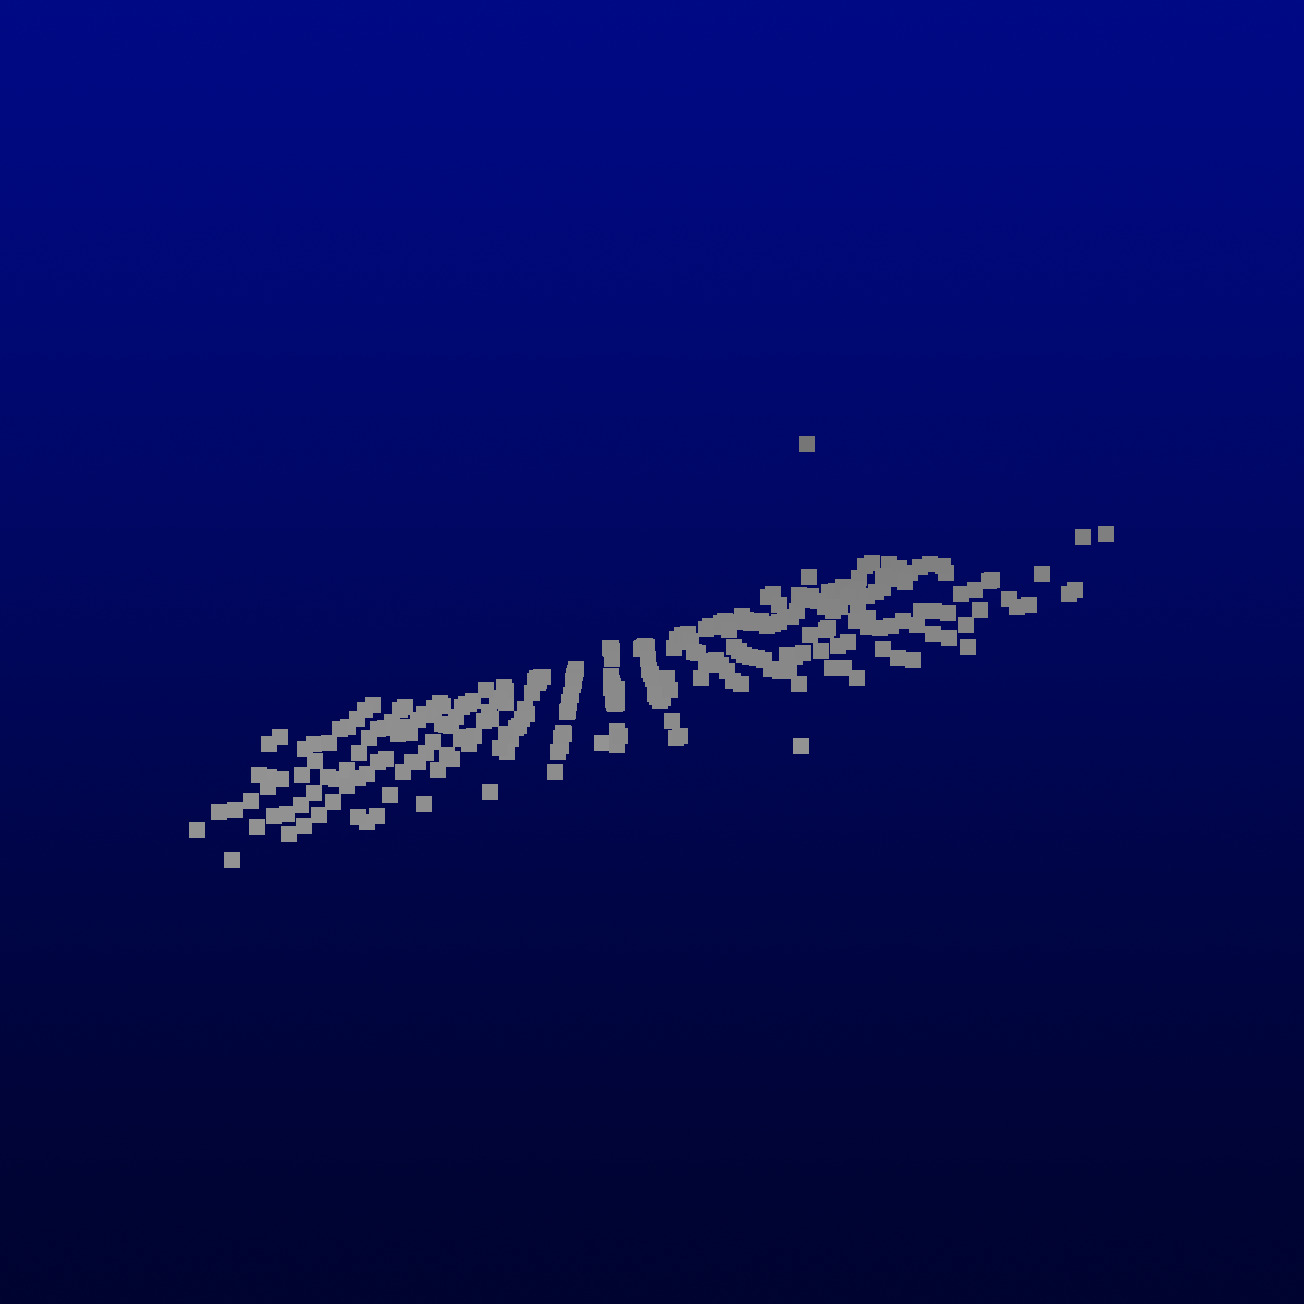
\includegraphics[width=4cm]{img/pointclouds/pcl_sample_top}
	& 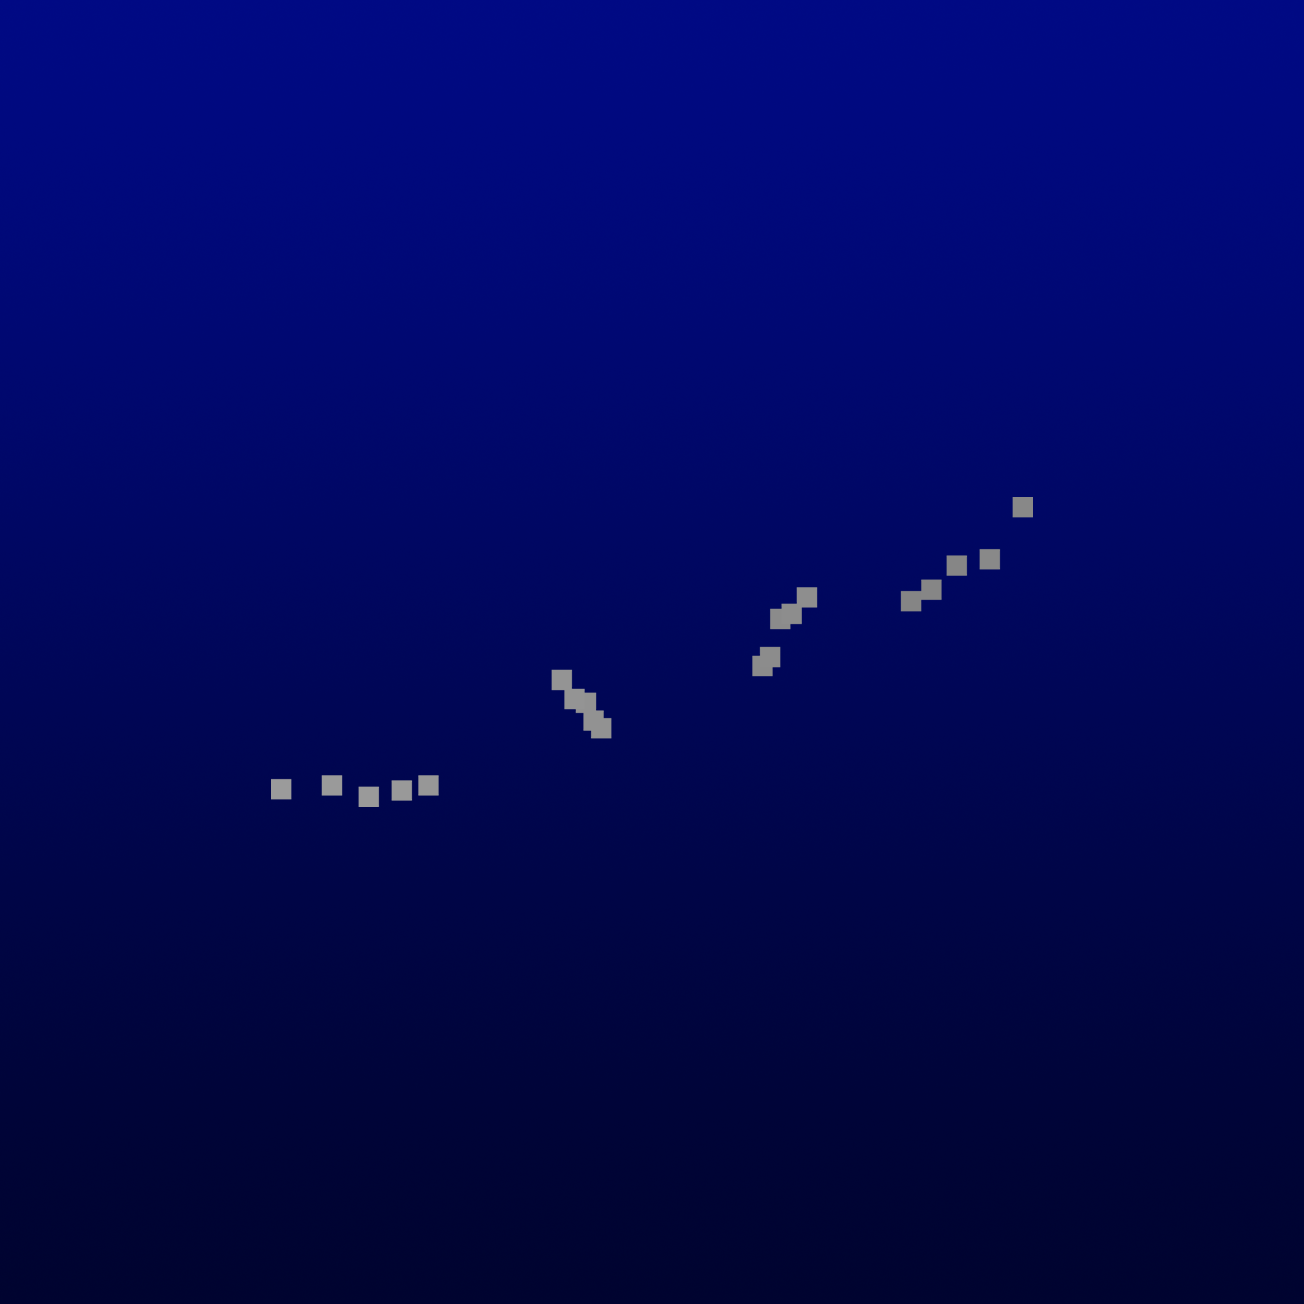
\includegraphics[width=4cm]{img/pointclouds/pcl_sub_top}
\end{tabular}
\caption{Gespeicherte Hindernis Punktwolke desselben Objektes beider Methoden.}
\label{fig:obstacle_pointclouds}
\end{table}

\noindent
Prinzipiell ist die Punktwolke der \emph{Samplepoint Detecion} aufgrund der Verwendung von signifikant mehr Messpunkten wesentlich detaillierter. Dies kann beispielsweise bei einer dreidimensionalen Kartographierung von Vorteil sein. Jedoch wäre es auch möglich, das aufgrund der kleinen Fläche mehr Ausreißer  erkannt werden. Dies konnte zwar im Rahmen der Tests nur bei spiegelnden und durchsichtigen Flächen beobachtet werden, ist jedoch eine prinzipiell mögliche Fehlerquelle bei der späteren Hindernisvermeidung.\\

%%% BEWEGUNGEN GUT FUER DIE ERKENNUNG DURCH BEIDE METHODEN
\noindent
Weiterhin ließ sich während der Versuchsdurchführung deutlich erkennen, dass Bewegungen einen großen Einfluss auf die Hinderniserkennung haben. Wurden die Hindernisse bewegt, konnte gerade im Fall der \textit{Subimage Detection} festgestellt werden, dass die Erkennung kleiner Hindernisse signifikant besser funktionierte. Dadurch eliminieren sich bereits beschriebene Konfliktfälle in denen sich das zu erkennende Hindernis an der Kreuzung mehrerer \textit{Subimages} befand. Die Bewegung sorgte in diesem Fall dafür das die Hindernisse in mehr Frames erkannt wurden als in einer statischen Szene. Selbiges Phänomen trat auch bei der \textit{Samplepoint Detection} auf.\\


